\documentclass[a4paper]{article}

\usepackage[utf8]{inputenc}
\usepackage[top=1.5cm, bottom=1.5cm, left=1.5cm, right=1.5cm]{geometry}
\usepackage[pdftex]{graphicx}
\usepackage{color}
\usepackage{makeidx}
\usepackage{subfig}
\usepackage{float}



\newcommand{\HRule}{\rule{\linewidth}{0.5mm}}
\newcommand{\tab}{\hspace*{2em}}
\makeindex
\begin{document}

\begin{titlepage}



\begin{center}

{\vspace*{8.5cm}}

% Upper part of the page


\textsc{\LARGE University of Aberystwyth}\\[1.5cm]

\textsc{\Large First year group project}\\[0.5cm]


% Title
\HRule \\[0.4cm]
{ \huge \bfseries UML2 Java}\\[0.4cm]

\HRule \\[1.5cm]

% Author and supervisor
\begin{minipage}{0.4\textwidth}
\begin{center} \large
\emph{Authors:}\\
Daniel Mal\'{y},\\ Samuel Sherar,\\ Lee Smith
\end{center}
\end{minipage}

\vfill


\end{center}

\end{titlepage}


\newcommand{\imagespace}[0]{\ \ \ \ \ \ \ }
\setlength\fboxsep{0pt}
\setlength\fboxrule{0.7pt}
%\includegraphics[trim= left bottom right top, clip, scale]

\begin{center}\huge{UML2Java Graphical Designer}
\end{center}

\texttt{UML2Java} is a Graphic User Interface program that allows a user to create UML2 class diagrams. The program will then output the class files from the created class diagram including all relevant fields, methods and relationships to
other classes. The UML designer was created as a requirement for our first year group project.

\newpage
\tableofcontents 
\newpage

\section{File Menu} 

\subsection{Create new Class Diagram} \index{File!Create New diagram}
To create a new Class Diagram, go to the top menu bar and press \texttt{File $\rightarrow$ New}
\begin{figure}[H] \begin{center} 
\fbox{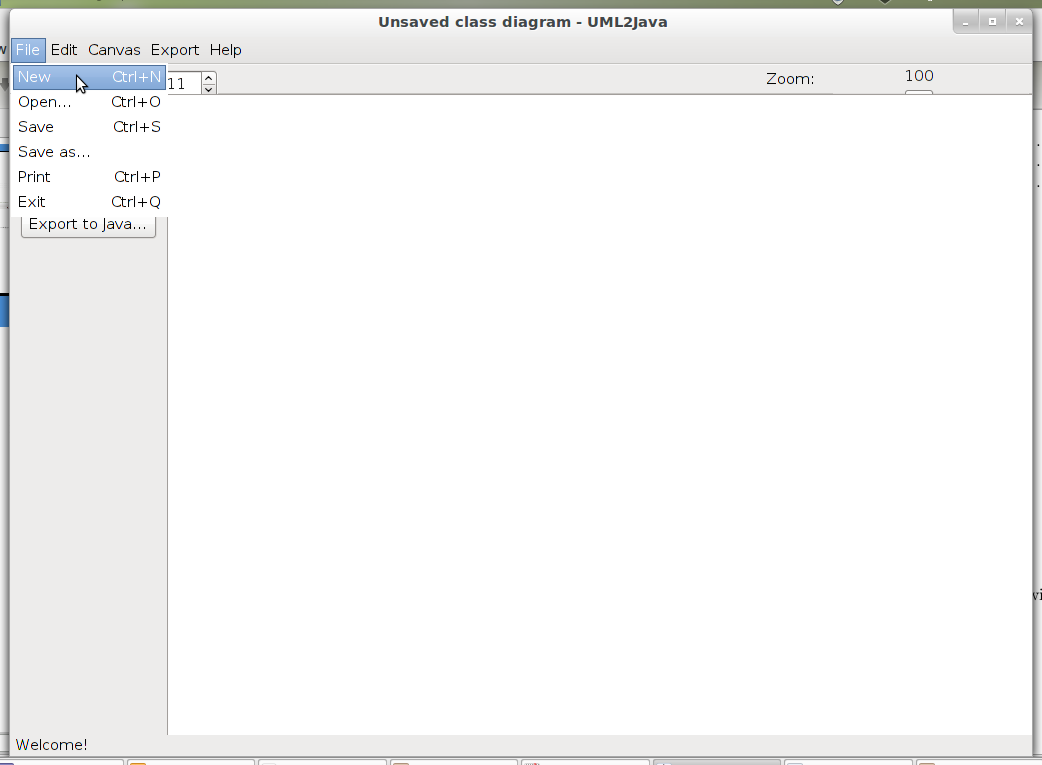
\includegraphics[trim = 0pt 200pt 0pt 0pt, clip, scale=1.2]{./images/file-new.png}}
\caption{Creating a new Diagram} \vspace{-20pt}
\end{center} \end{figure}

\subsection{Open an existing diagram} \index{File!Open Saved diagram}
To open a previously saved diagram, go to the top menu bar and press \texttt{File $\rightarrow$ Open...} or simply press \texttt{CTRL+O}
This will open up a new window asking for the location of the file you wish to open

\begin{center} \begin{figure}[H]
\vspace{-20pt}
\subfloat[File $\rightarrow$ Open]{\label{fig:open}\fbox{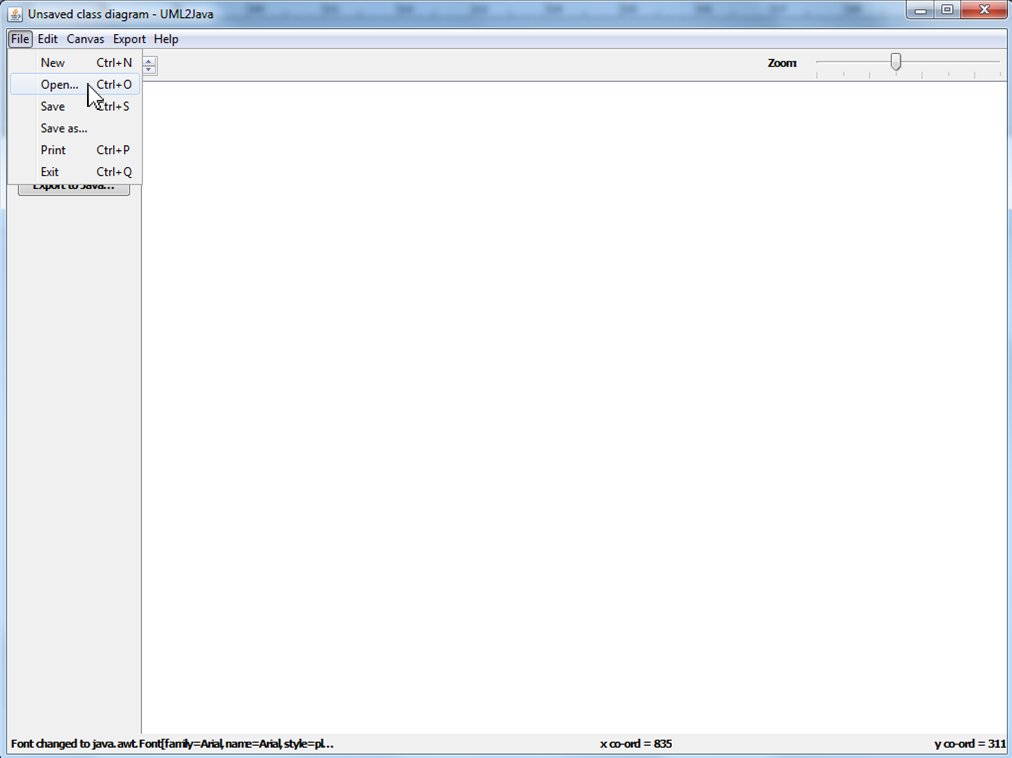
\includegraphics[trim = 0pt 200pt 250pt 0pt, clip, scale=1.2]{./images/file-open1.png}}\imagespace}
\subfloat[Select File to open]{\label{fig:openSelect}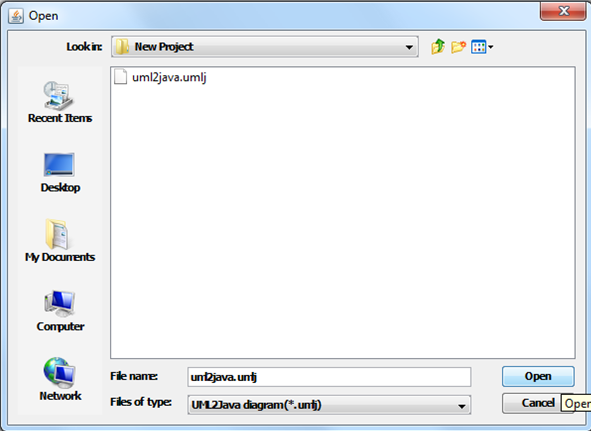
\includegraphics[scale=1]{./images/file-open2.png}}
\caption{Opening an existing diagram} 
\vspace{-20pt}
 \end{figure} \end{center}

\subsection{Saving a diagram} \index{File!Saving}
To save a diagram, go to the top menu bar and press \texttt{File $\rightarrow$ Save/Save as...} or simply press \texttt{CTRL+S}

\begin{center} \begin{figure}[H]
\vspace{-20pt}
\subfloat[File $\rightarrow$ Save] {\label{fig:save}\fbox{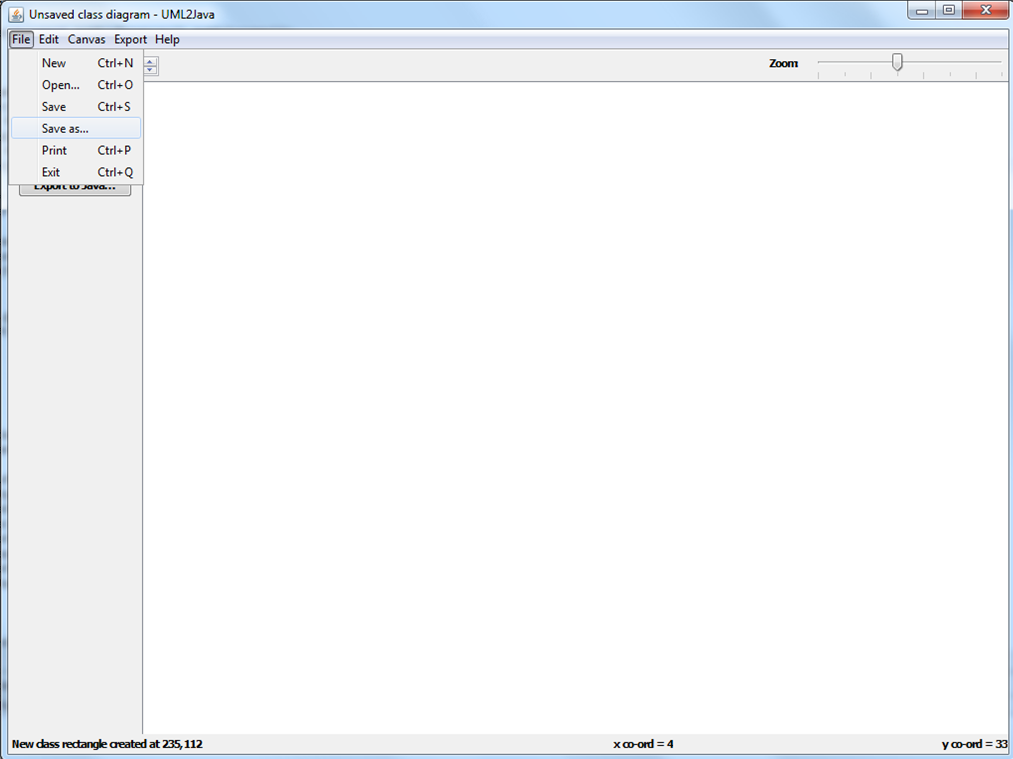
\includegraphics[trim = 0pt 200pt 250pt 0pt, clip, scale=1.2]{./images/file-save1.png}}\imagespace} 
\subfloat[Select Save Location]{\label{fig:saveSelect}\fbox{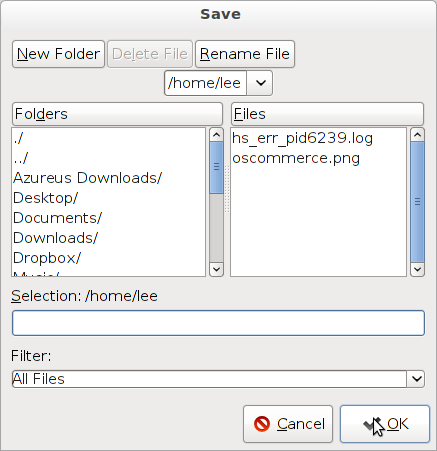
\includegraphics[scale=1]{./images/file-save2.png}}}
\caption{Saving a diagram} \vspace{-20pt} 
\end{figure} \end{center}

\subsection{Printing a Diagram} \index{File!Printing}
To print a created diagram, go to the top bar and press \texttt{File $\rightarrow$ Print} or simply press \texttt{CTRL+P} and select the desired printer from the open window

\begin{figure}[H] \begin{center} 
\vspace{-20pt}
\subfloat[File $\rightarrow$ Print] {\label{fig:print}\fbox{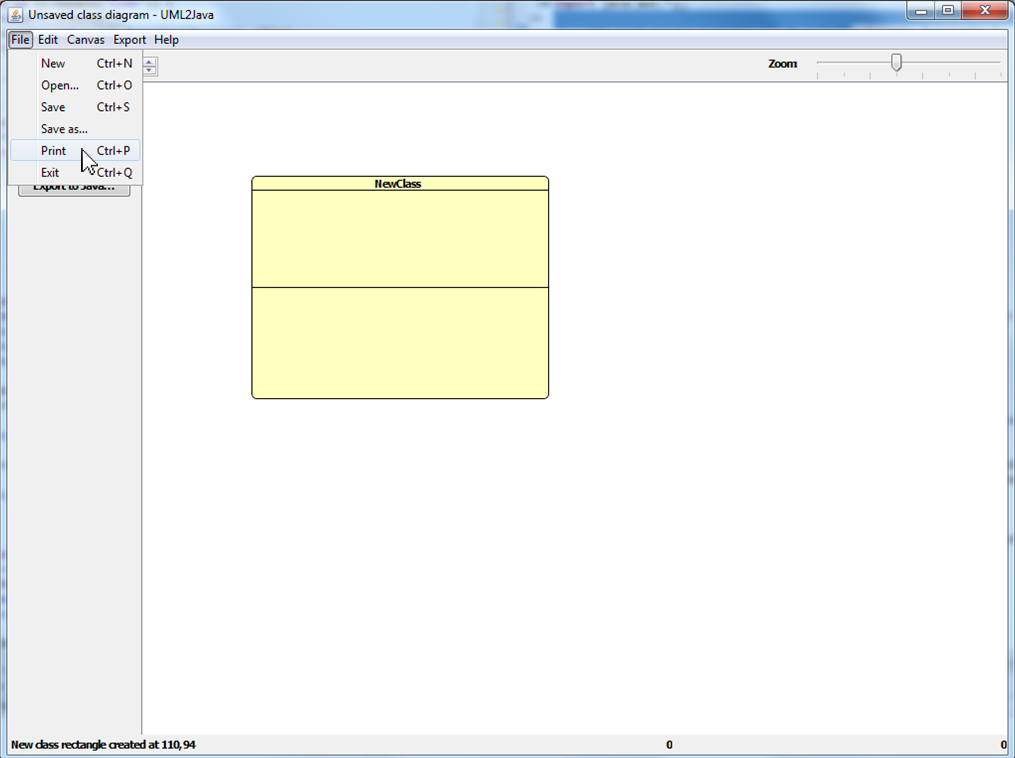
\includegraphics[trim = 0pt 200pt 250pt 0pt, clip, scale=1.2]{./images/file-print1.png}}\imagespace} 
\subfloat[Select Printer]{\label{fig:printerSelect}\fbox{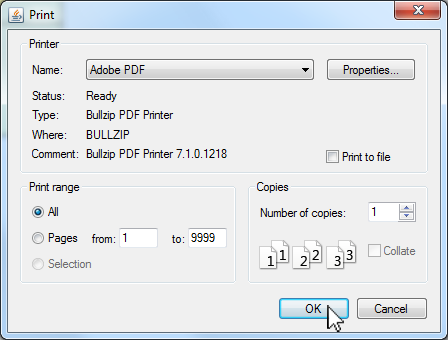
\includegraphics[scale=0.6]{./images/file-print2.png}}}
\caption{Printing a diagram} \vspace{-20pt} 
\end{center} \end{figure}

\subsection{Exiting the Designer} \index{File!Exiting UML2Java}
To end the current session in \texttt{UML2Java}
\begin{figure}[H] \begin{center} 
\label{fig:exit}\fbox{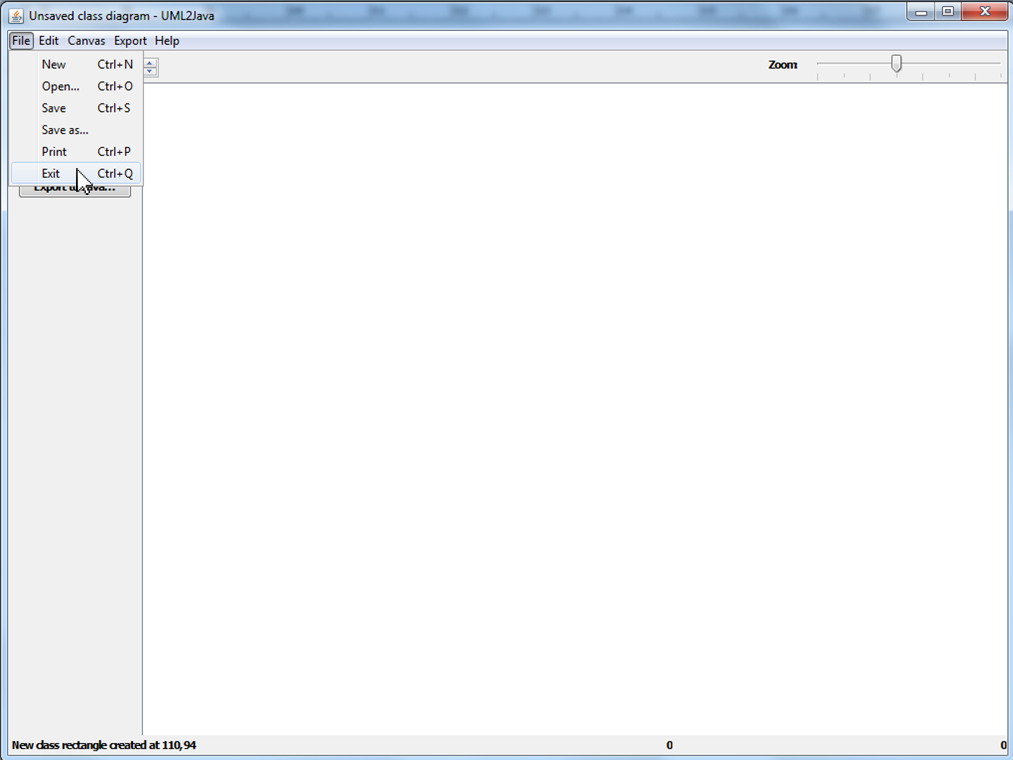
\includegraphics[trim = 0pt 200pt 300pt 0pt, clip, scale=1.2]{./images/file-exit.png}}
\caption{Exiting the Designer}
\vspace{-20pt}
\end{center} \end{figure}

\section{Edit Menu}
\subsection{Undoing an Action} \index{Edit!Undo}
If you require to undo the previous action, go to the top bar and press \texttt{Edit $\rightarrow$ Undo} or press \texttt{CTRL+Z} from the keyboard
\begin{figure}[H] \begin{center} 
\label{fig:undo}\fbox{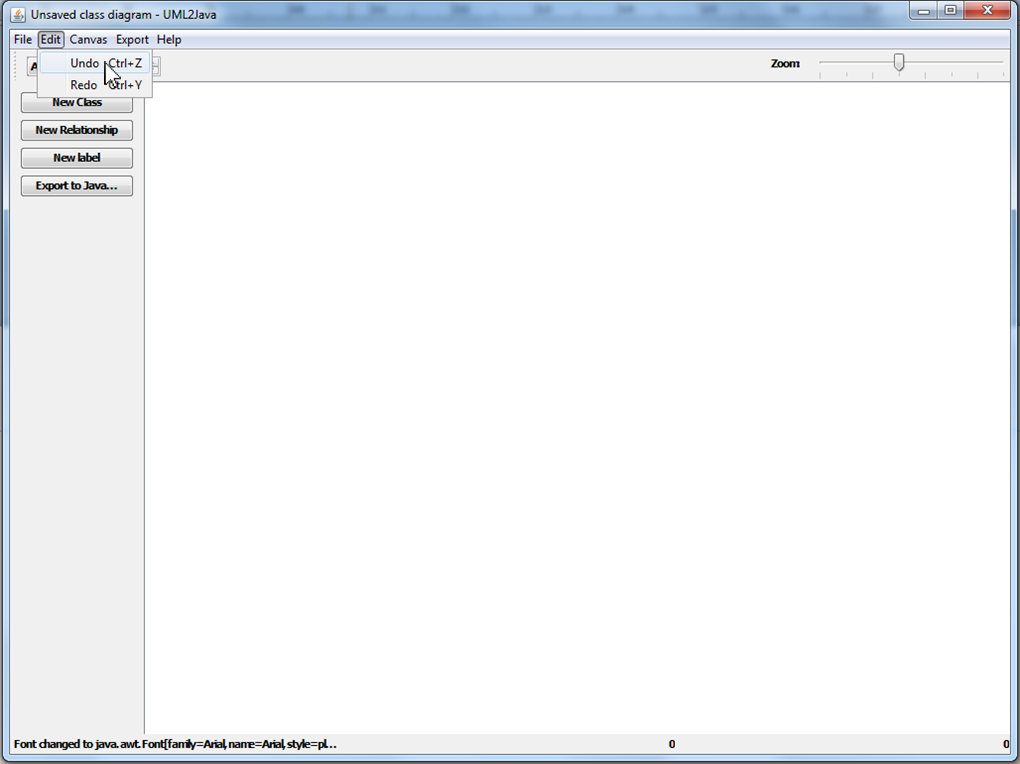
\includegraphics[trim = 0pt 200pt 300pt 0pt, clip, scale=1.2]{./images/edit-undo.png}}
\caption{Undo last Action}
\vspace{-20pt}
\end{center} \end{figure} 
\newpage
\subsection{Redoing an Action} \index{Edit!Redo}
if you need to redo a previously undone action, simply go to the top bar and press \texttt{Edit $\rightarrow$ Redo} or press \texttt{CTRL+Y} from your keyboard

\begin{figure}[H] \begin{center} 
\label{fig:redo}\fbox{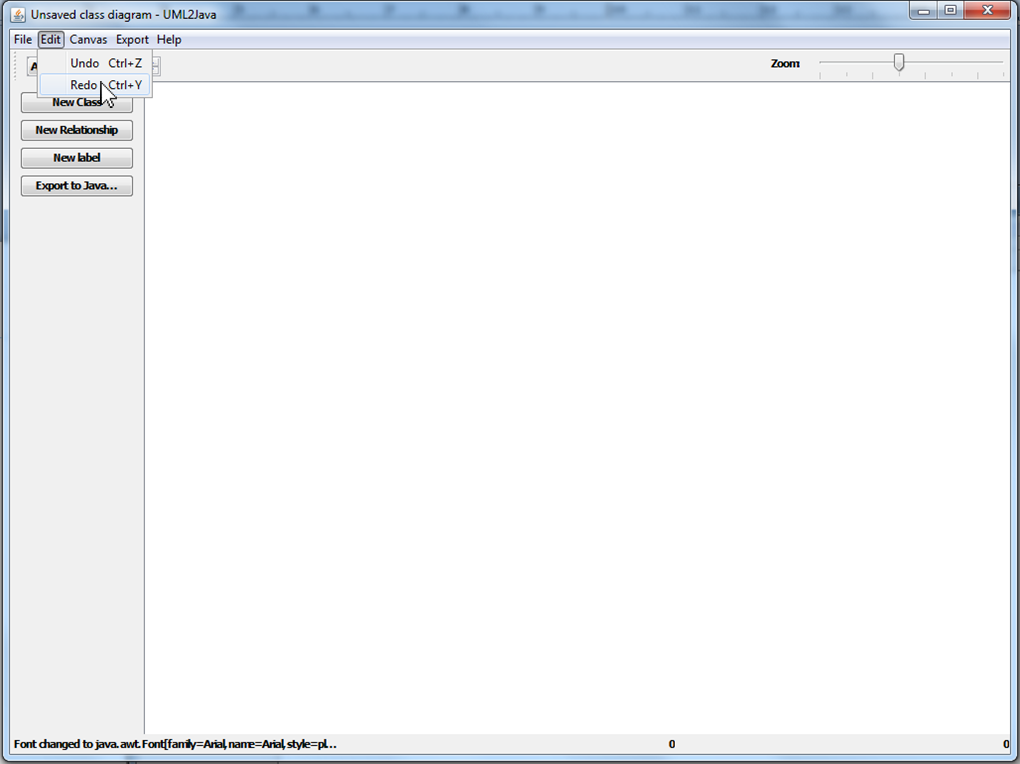
\includegraphics[trim = 0pt 200pt 300pt 0pt, clip, scale=1.2]{./images/edit-redo.png}}
\caption{Redoing an Action}
\vspace{-20pt}
\end{center} \end{figure} 

\section{Editing Canvas Settings}
\subsection{Resize the Canvas} \index{Canvas Settings!Resize}
If you require a different canvas size , you can do this from the top menu, pressing \texttt{Canvas $\rightarrow$ Resize}

 \begin{figure}[H] \begin{center}
\subfloat[Canvas $\rightarrow$ Resize...] {\label{fig:resizeOption}\fbox{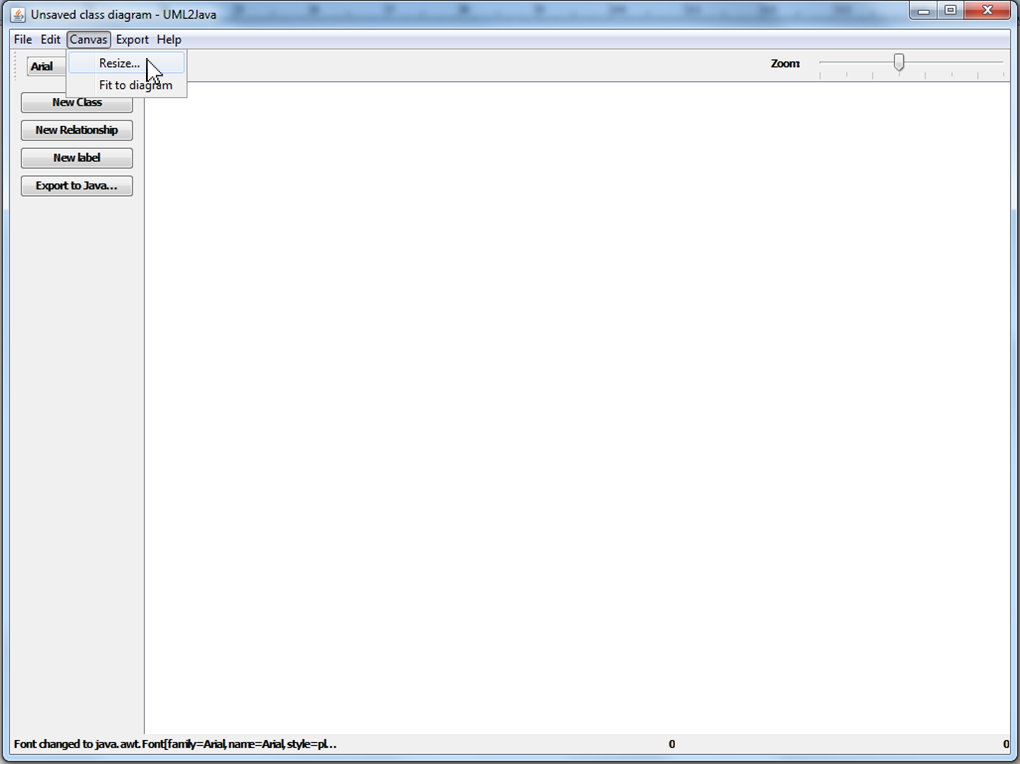
\includegraphics[trim = 0pt 200pt 250pt 0pt, clip, scale=1.2]{./images/canvas-resize1.png}}\imagespace} 
\subfloat[Select resize options]{\label{fig:resizeSet}\fbox{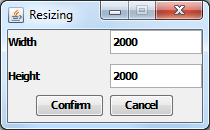
\includegraphics[scale=1]{./images/canvas-resize2.png}}}
\caption{Printing a diagram} \vspace{-20pt} 
\end{center} \end{figure} 

\subsection{Fitting to Diagram} \index{Canvas Settings!Fit to Diagram}
The canvas menu option also allows you to resize the canvas to a state where all of the current contents of the diagram will be able to be seen with little white space around the resulting design, to achieve this press \texttt{Canvas
$\rightarrow$ Fit to Diagram}
\begin{figure}[H] \begin{center}

\label{fig:fitDiagram}\fbox{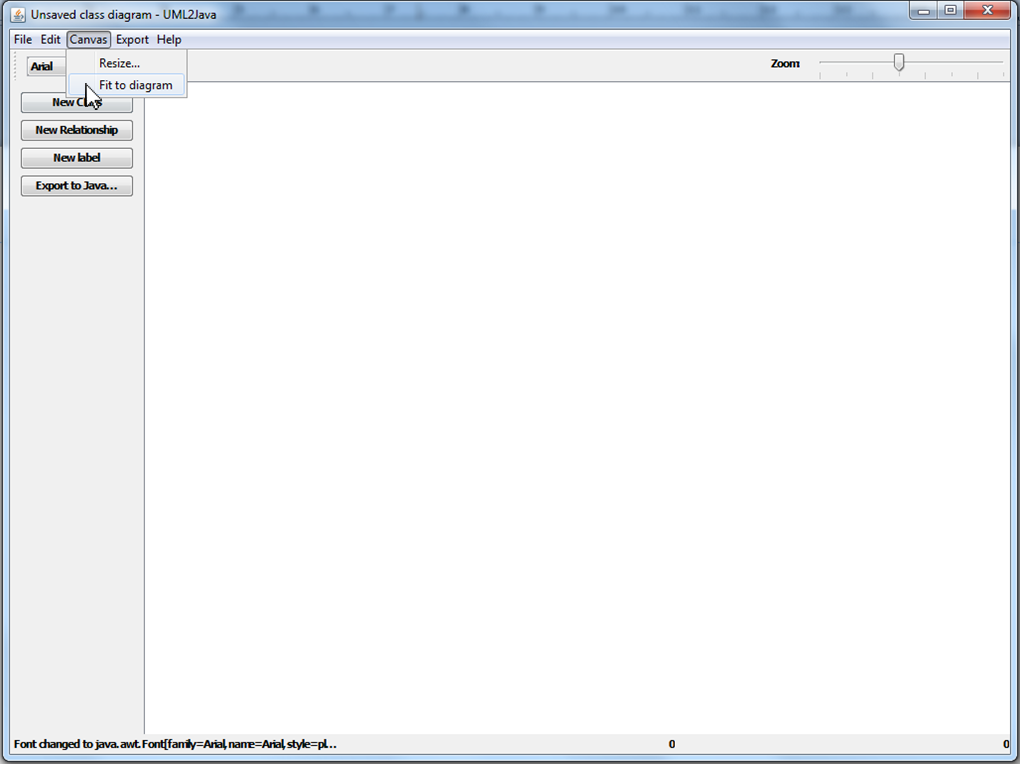
\includegraphics[trim = 0pt 200pt 250pt 0pt, clip, scale=1.2]{./images/canvas-fit.png}}
\caption{Fit diagram to visible canvas}
\vspace{-20pt}
\end{center} \end{figure} 
\newpage
\section{Exporting}
\subsection{Export to Code} \index{Exporting!Code}
To create the code files of your created diagram, go to the top bar and select \texttt{Export $\rightarrow$ Code} this will generate the .java files of your created diagram, it will take into account any relationships you have created
between classes, any variable declarations you have made, and methods you have created. Or you can go to the left menu bar and select \texttt{Export to Java} from the list there

\begin{figure}[H] \begin{center}
\subfloat[Export $\rightarrow$ Code] {\label{fig:exportcode}\fbox{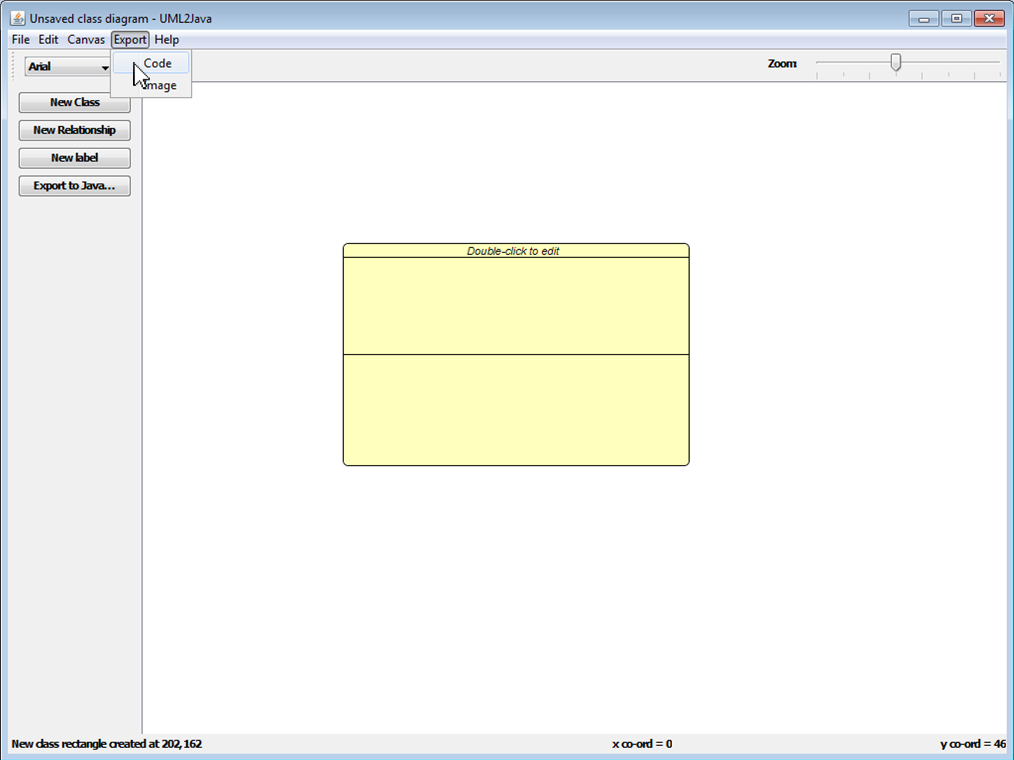
\includegraphics[trim = 0pt 200pt 250pt 0pt, clip, scale=1.075]{./images/export-code1.png}}} \imagespace
\subfloat[Export to Java...] {\label{fig:exportJava}\fbox{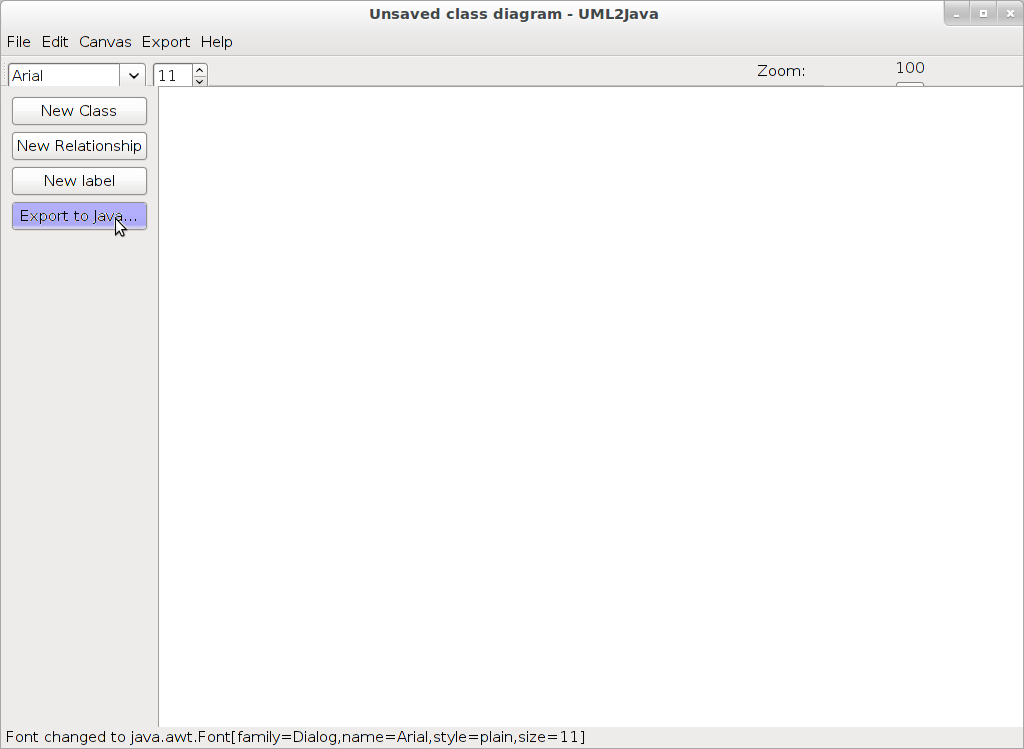
\includegraphics[trim = 0pt 355pt 450pt 0pt, clip, scale=0.6]{./images/export-code2.png}}} \end{center}
You will then be asked to select a directory to save the code files to, you can select a existing directory or create a new one
\begin{center}
\subfloat[Choose Directory to create files] {\label{fig:exportJavaDirectory}\fbox{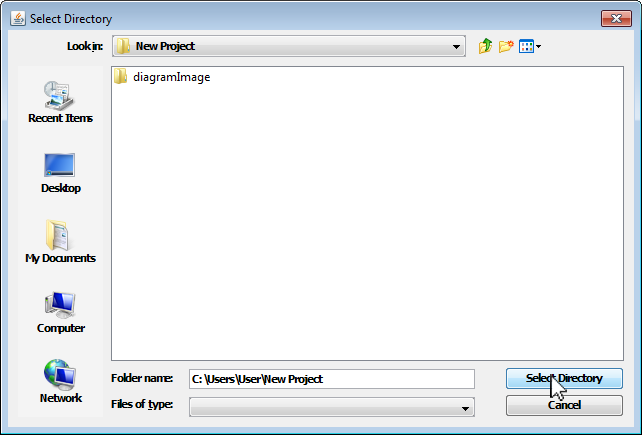
\includegraphics[trim = 0pt 0pt 0pt 0pt, clip, scale=0.45]{./images/export-code-directory.png}}}
\caption{Exporting to Java code}
\end{center}
\vspace{-20pt}
\end{figure}

\subsection{Export Image of Diagram}\index{Exporting!Image}
To create an image file of the class diagram you have created, go to \texttt{Export $\rightarrow$ Image} and an save box will appear, where you can select the location of where you wish to save the file and also the file type, either
\texttt{.png} or \texttt{.jpg}
\begin{figure}[H]
\begin{center}
\subfloat[Export $\rightarrow$ Image] {\label{fig:exportImage}\fbox{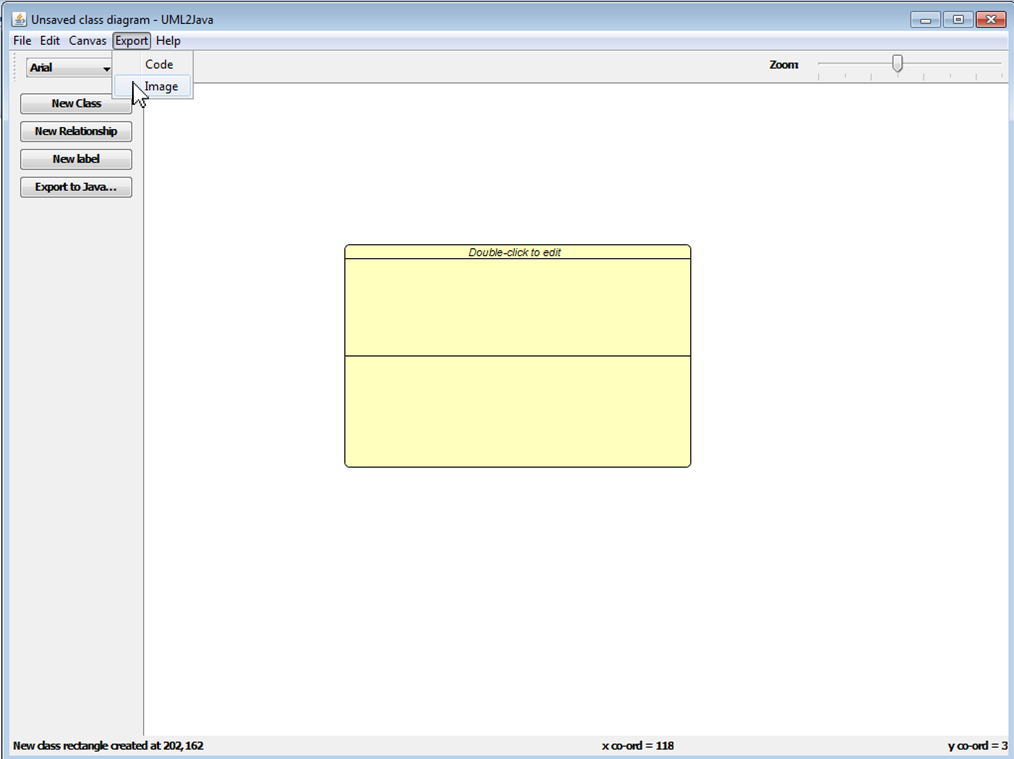
\includegraphics[trim = 0pt 200pt 250pt 0pt, clip, scale=1.2]{./images/export-image1.png}}} \imagespace
\subfloat[Choose Directory to save image] {\label{fig:exportImageLoc}\fbox{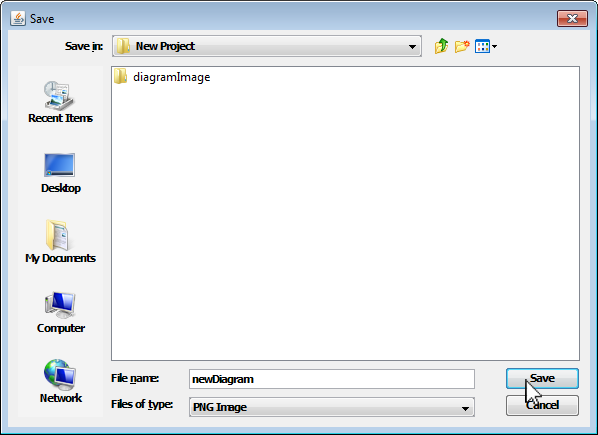
\includegraphics[trim = 0pt 0pt 0pt 0pt, clip, scale=0.5]{./images/export-image2.png}}}
\caption{Export Diagram as Image}
\end{center}
\end{figure}

\newpage

\section{Adding Elements to the Class Diagram}
\subsection{Adding a new class}\index{Adding to diagram!Classes}
To create a new class on the diagram, go to the left-hand menu and select \texttt{New Class}
\begin{figure}[H]
\begin{center}
	\subfloat[Add new class] {\label{fig:addClass1}\fbox{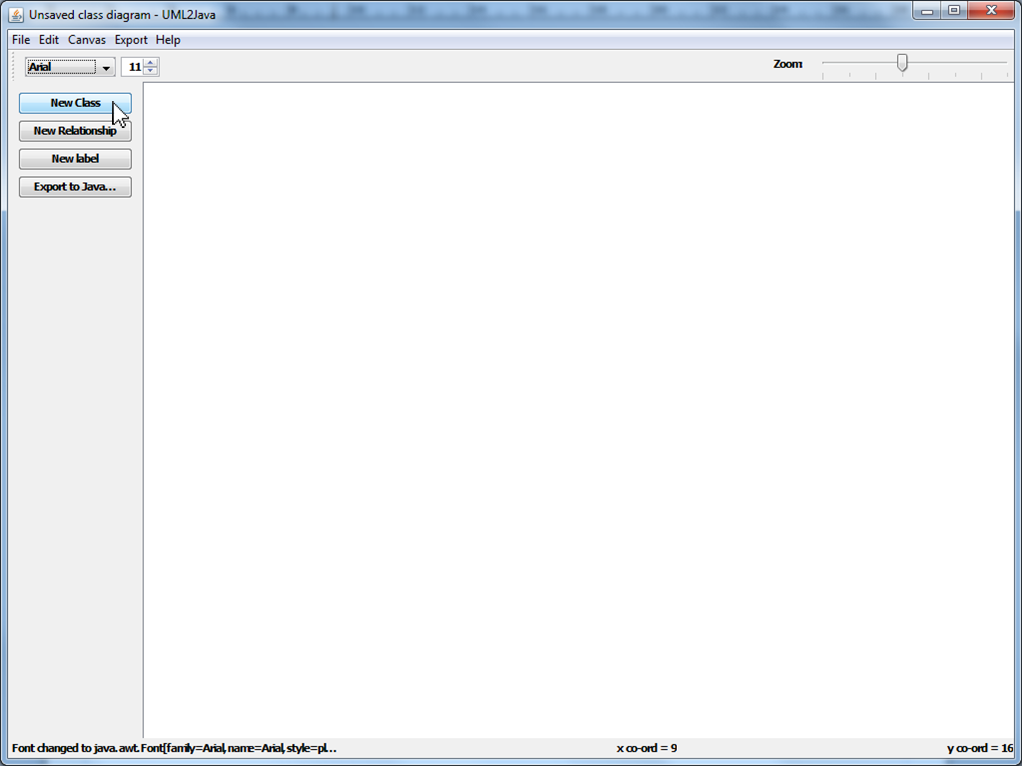
\includegraphics[trim = 0pt 350pt 450pt 0pt, clip, scale=0.6]{./images/addNewClass1.png}}}
\end{center}

To make sure that you have selected to add a new class, once pressed, a message will appear in the status bar at the bottom of the window
\begin{center}
\subfloat[Click to create new class] {\label{fig:addClass2}\fbox{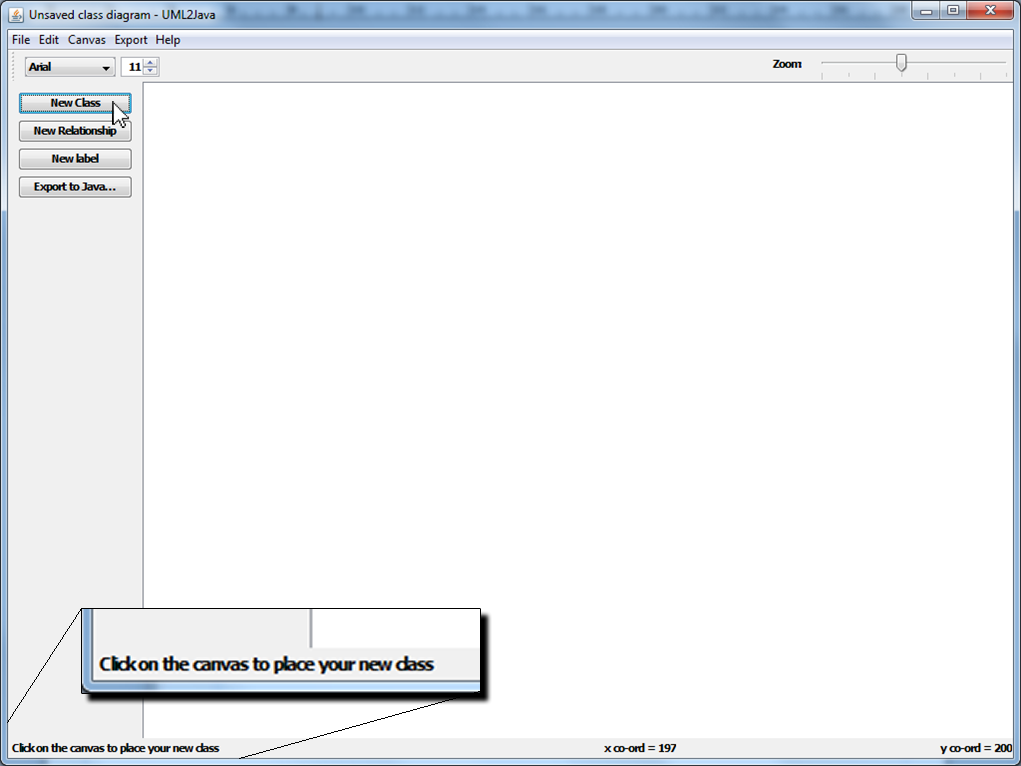
\includegraphics[trim = 0pt 0pt 300pt 300pt, clip, scale=0.4]{./images/addNewClass2.png}}}
\end{center}

To add the class to the diagram, left-click on the white canvas and your new class will appear

\begin{center}
\subfloat[Added Class]{\label{fig:addClass3}\fbox{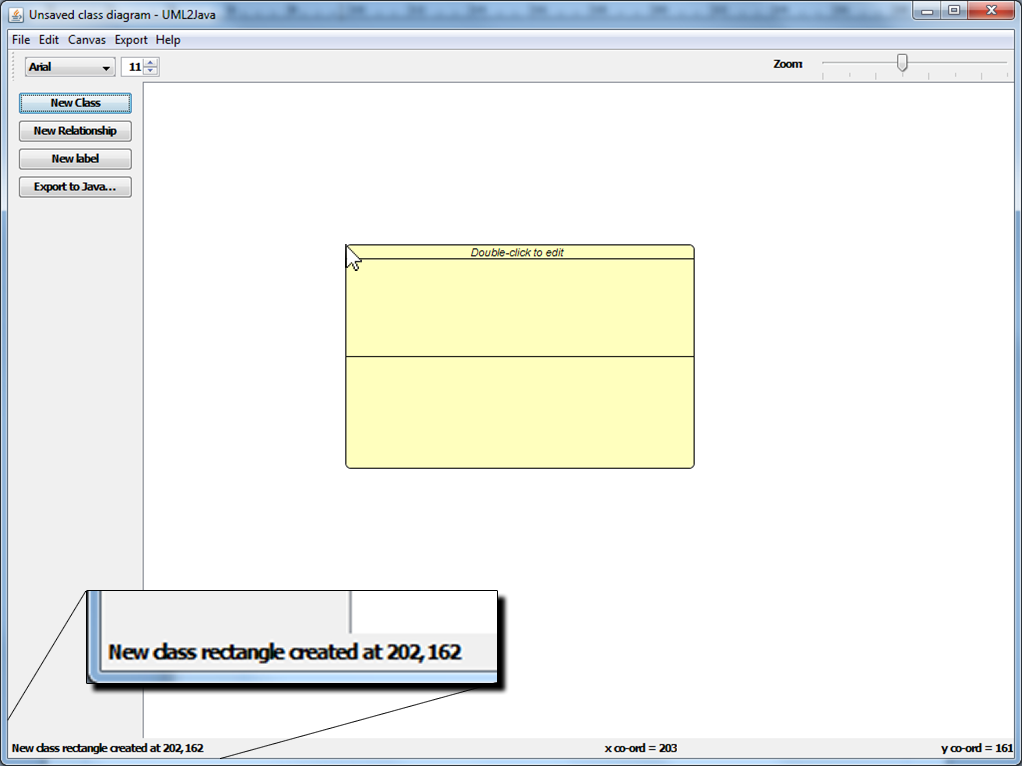
\includegraphics[scale=0.4]{./images/addNewClass3.png}}} \end{center}

You will recieve confirmation via the status bar at the bottom of the screen, giving the x and y co-ordinates of the generated class box
\caption{Adding a new class to diagram}
\vspace{-10pt}
\end{figure}
\newpage
\subsubsection{Adding Data fields to the new Class}\index{Adding to diagram!Data Fields/Variables}
To add a new Data field to the Created Class, \texttt{Right Click} on the class, and select \texttt{Add data field}, the new data field will then be added to the diagram.
\begin{figure}[H]
\begin{center}
\subfloat[Right-Click $\rightarrow$ Add data field] {\label{fig:addData}\fbox{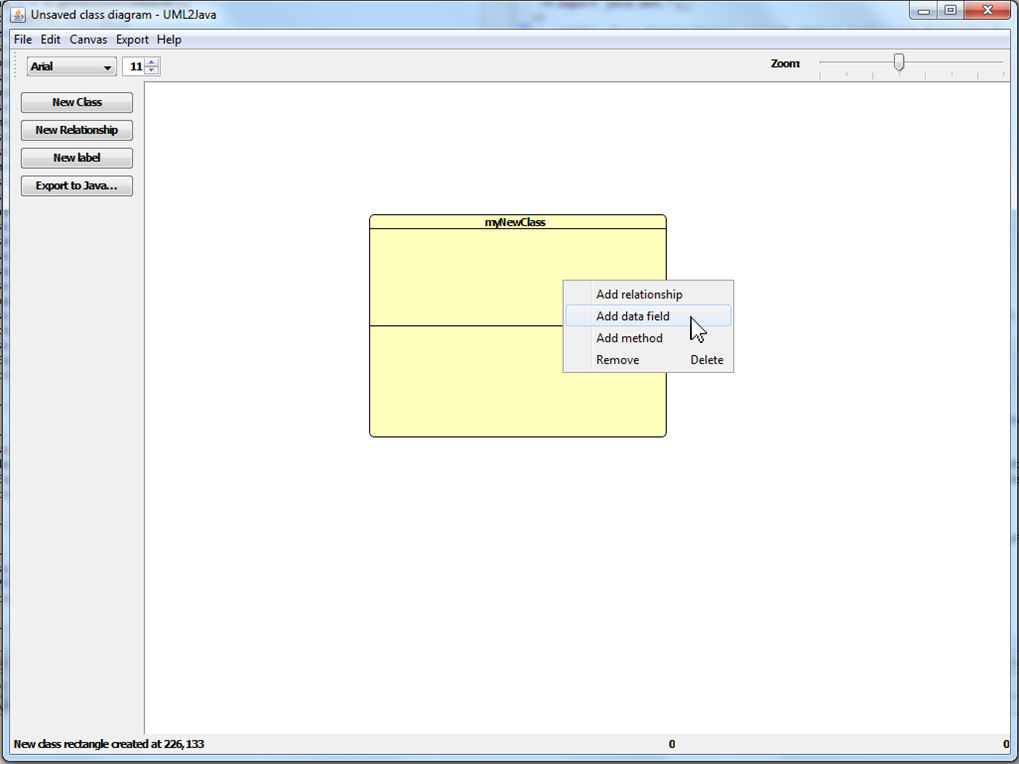
\includegraphics[trim = 105pt 100pt 95pt 60pt, clip, scale=1]{./images/addDataField1.png}}} \imagespace
\subfloat[Added Data Field] {\label{fig:addedData}\fbox{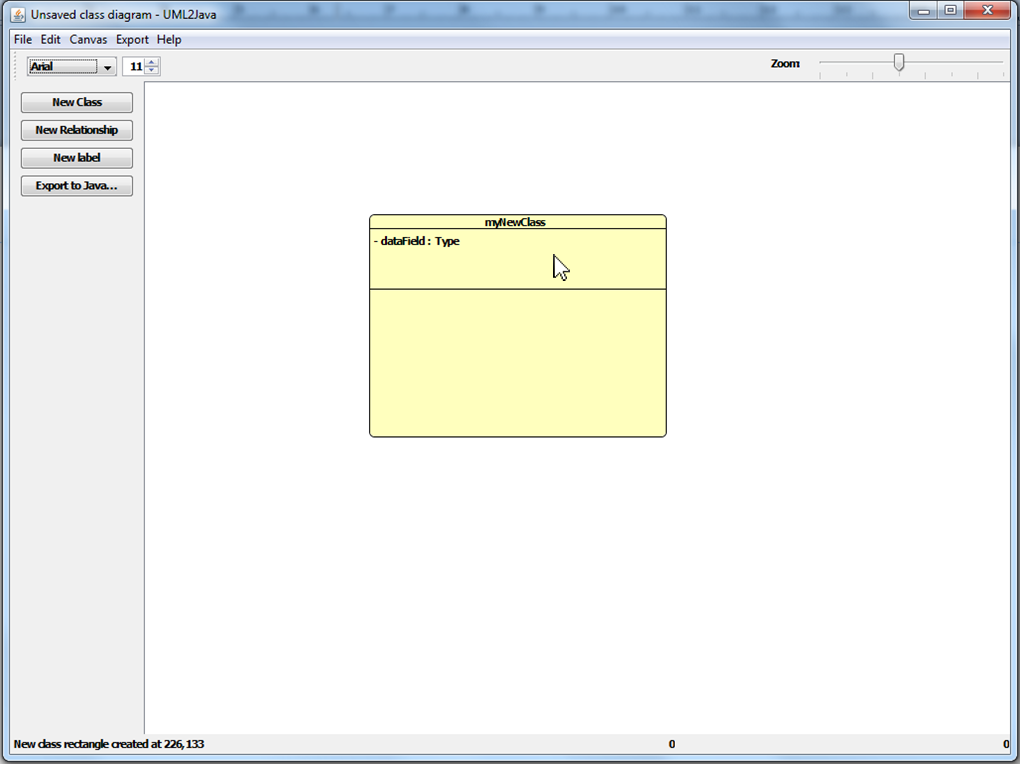
\includegraphics[trim = 105pt 100pt 95pt 60pt, clip, scale=1]{./images/addDataField2.png}}}
\caption{Adding a new Data Field to the Class}
\end{center}
\end{figure}

\subsubsection{Adding Methods to the new Class}\index{Adding to diagram!Methods}
to add a new method to the class, \texttt{Right Click} on the class, and select \texttt{Add method}, the new method will then be added to the diagram

\begin{figure}[H]
\begin{center}
\subfloat[Right-Click $\rightarrow$ Add Method] {\label{fig:addMethod}\fbox{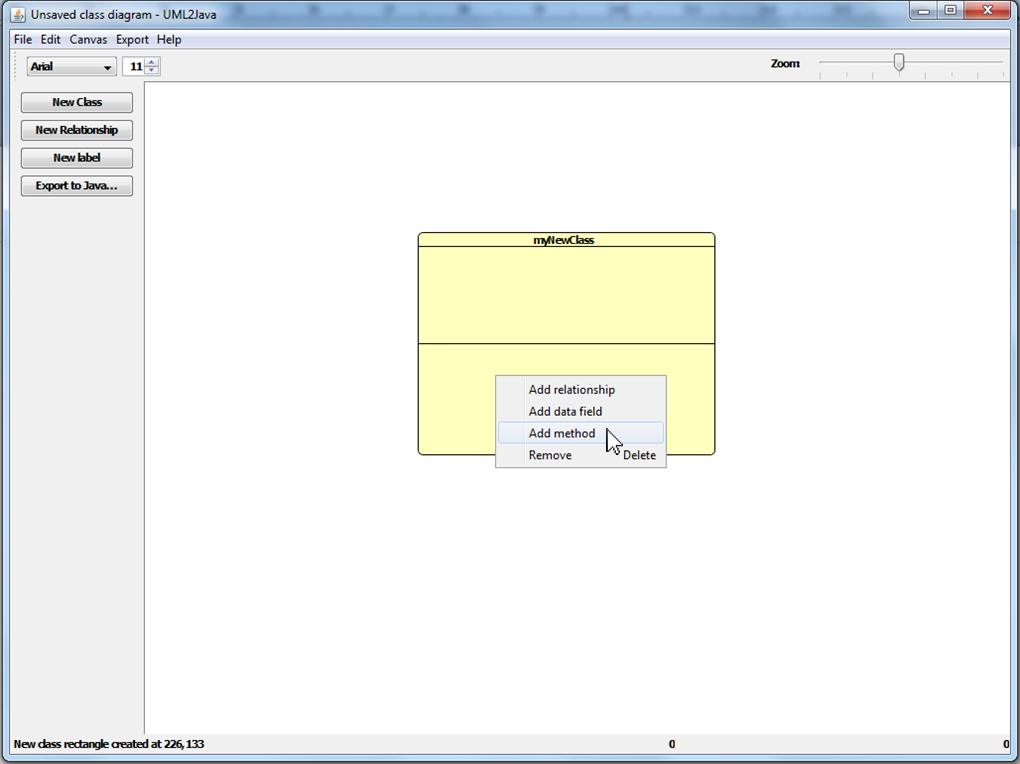
\includegraphics[trim = 125pt 100pt 75pt 60pt, clip, scale=1]{./images/addMethod1.png}}} \imagespace
\subfloat[Added Data Field] {\label{fig:addedMethod}\fbox{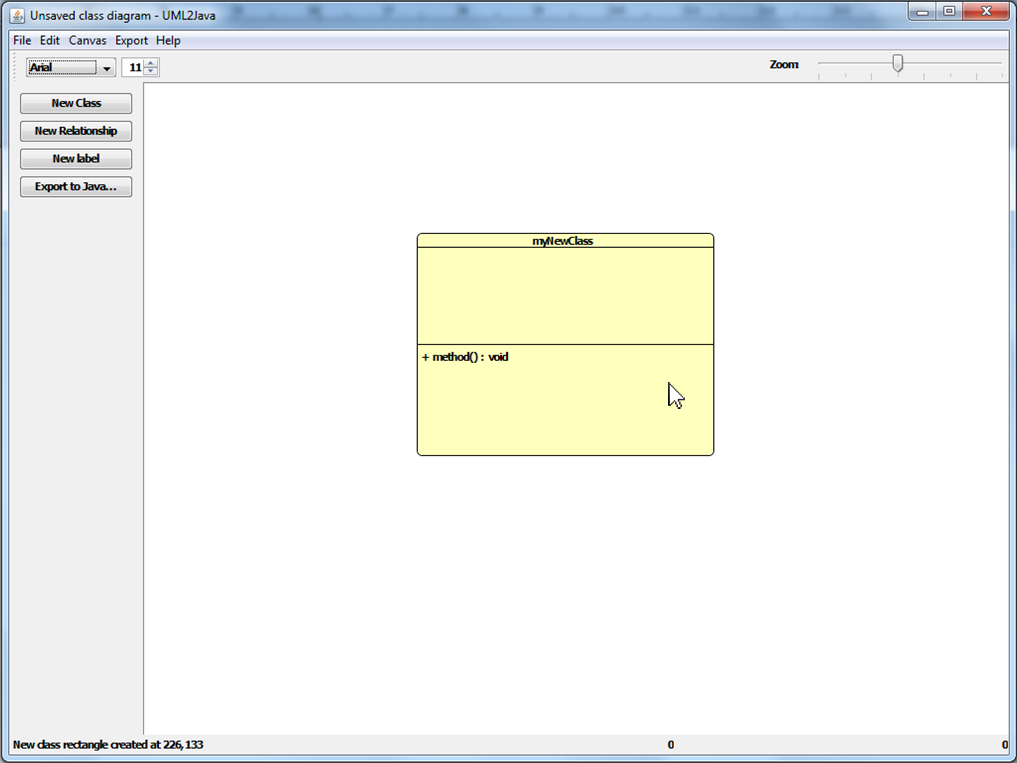
\includegraphics[trim = 125pt 100pt 75pt 60pt, clip, scale=1]{./images/addMethod2.png}}}
\caption{Adding a new Method to the Class}
\end{center}
\end{figure}

\newpage

\subsection{Adding a new Relationship between classes}\index{Adding to diagram!Relationships}
To add a relation\textbf{}ship between two classes, press \texttt{New Relationship} from the left-hand menu, or right click on a class to bring up a popup menu
\begin{figure}[H]
\begin{center}
\subfloat[Press New Relationship] {\label{fig:addRelationship1}\fbox{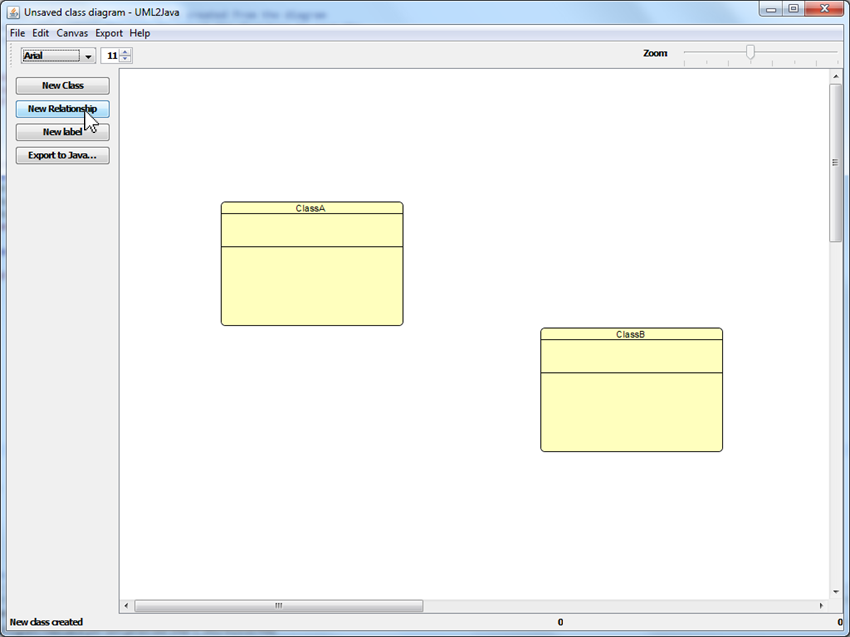
\includegraphics[trim = 0pt 200pt 250pt 0pt, clip, scale=1.075]{./images/addRelationship1.png}}} \imagespace
\subfloat[Right-Click $\rightarrow$ Add Relationship] {\label{fig:addRelationship2}\fbox{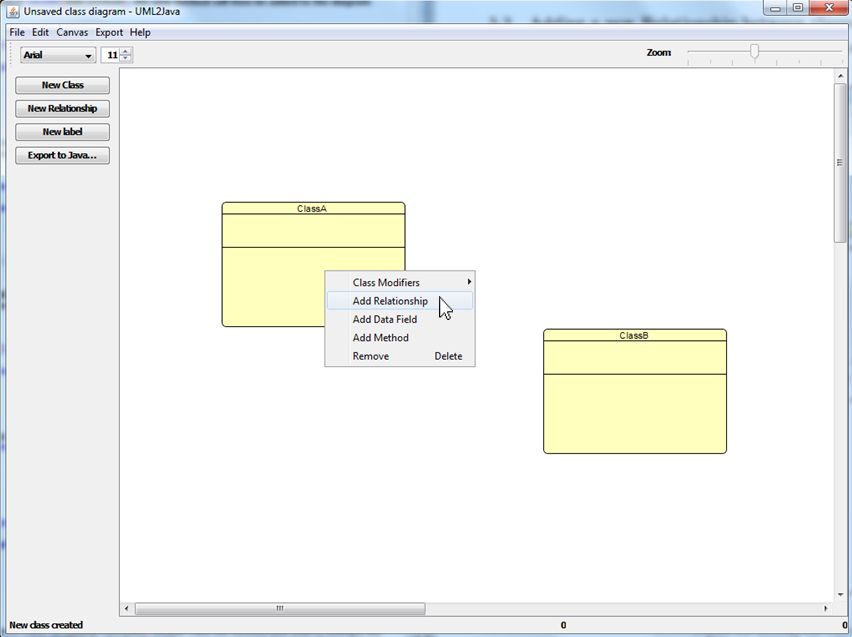
\includegraphics[trim = 60pt 120pt 140pt 80pt, clip, scale=1.075]{./images/addRelationship2.png}}}\\*
\end{center}

If you selected option a) then you will be required to press the inital class and the linking class. Option b) will automatically assume the class you used to \texttt{Add Relationship} is the inital class. The current state of
what needs to be selected will be displayed in the status bar at the bottom of the window.
\begin{center}

\subfloat[1st Class] {\label{fig:addRelationship3}\fbox{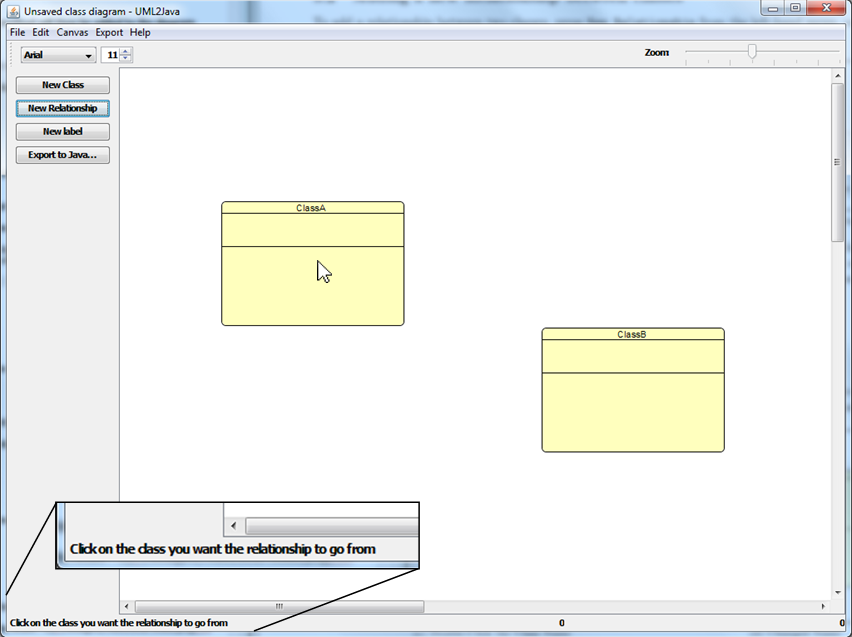
\includegraphics[trim = 0pt 0pt 0pt 0pt, clip, scale=0.55]{./images/addRelationship3.png}}} \imagespace
\subfloat[2nd Class] {\label{fig:addRelationship4}\fbox{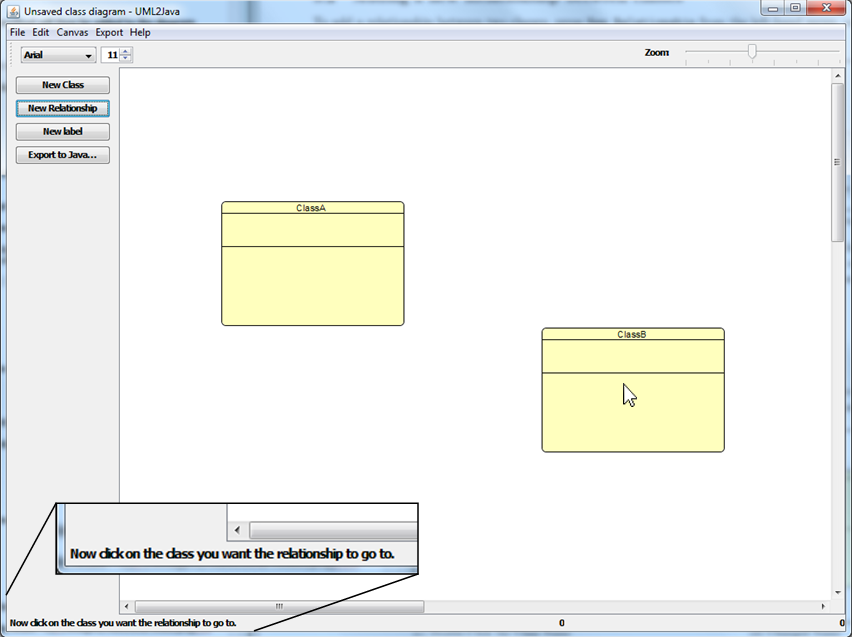
\includegraphics[trim = 0pt 0pt 0pt 0pt, clip, scale=0.55]{./images/addRelationship4.png}}}\\*
\end{center}
A arrow will then be drawn linking the two classes\\*
\begin{center}
\subfloat[Relationship Drawn] {\label{fig:addRelationship5}\fbox{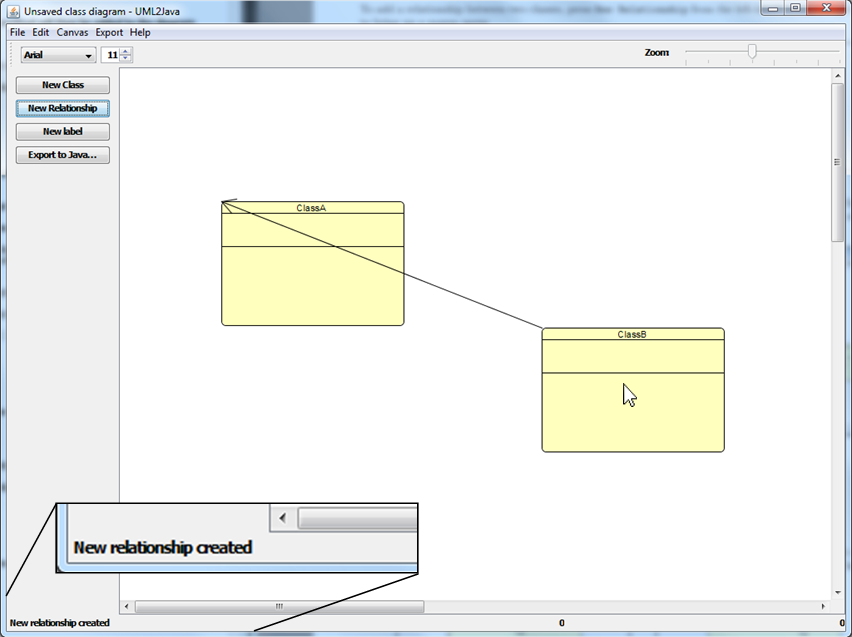
\includegraphics[trim = 0pt 0pt 0pt 0pt, clip, scale=0.8]{./images/addRelationship5.png}}}
\caption{Adding a realtionship between classes}
\end{center}
\end{figure}


\section{Editing}
\subsection{Changing the Class Name}\index{Editing!Class Name}
To change the class name of a class added to the diagram \emph{(see Adding new Class)} and Double-Click the class name, the text should highlight and you can then enter the new name, press return to confirm your new Class Name

\begin{figure}[H]
\begin{center}
\subfloat[Double-Click the Class Name] {\label{fig:editClassName}\fbox{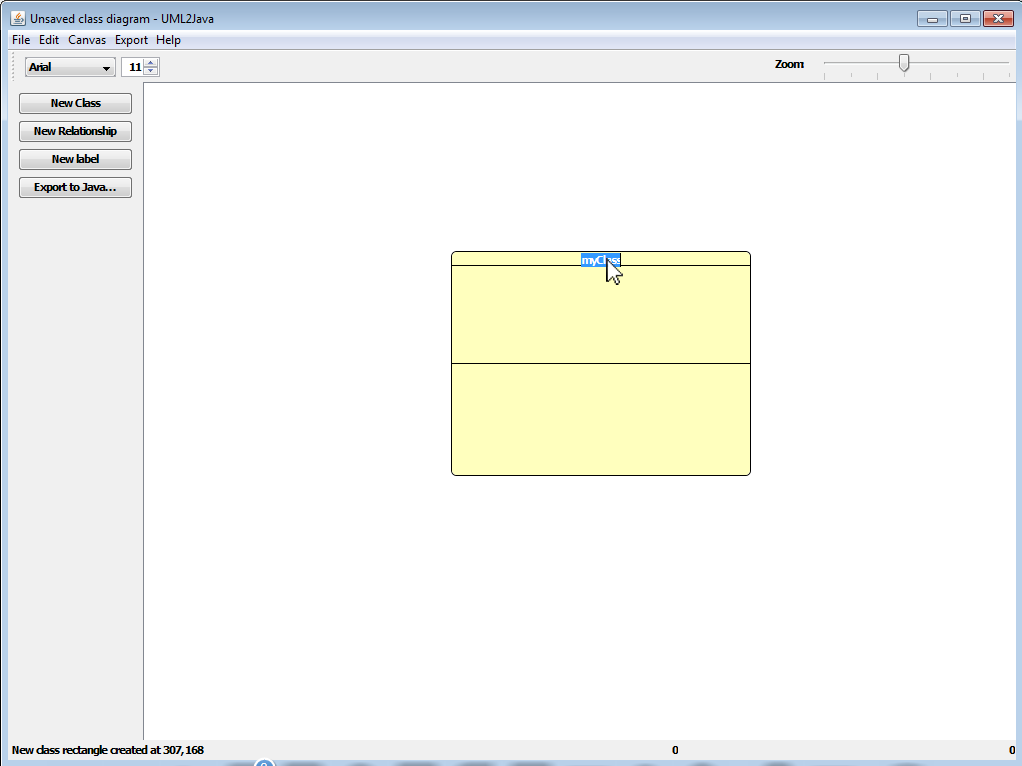
\includegraphics[trim = 135pt 90pt 65pt 70pt, clip, scale=1]{./images/editClassName1.png}}} \imagespace
\subfloat[Changed Name] {\label{fig:editedClassName}\fbox{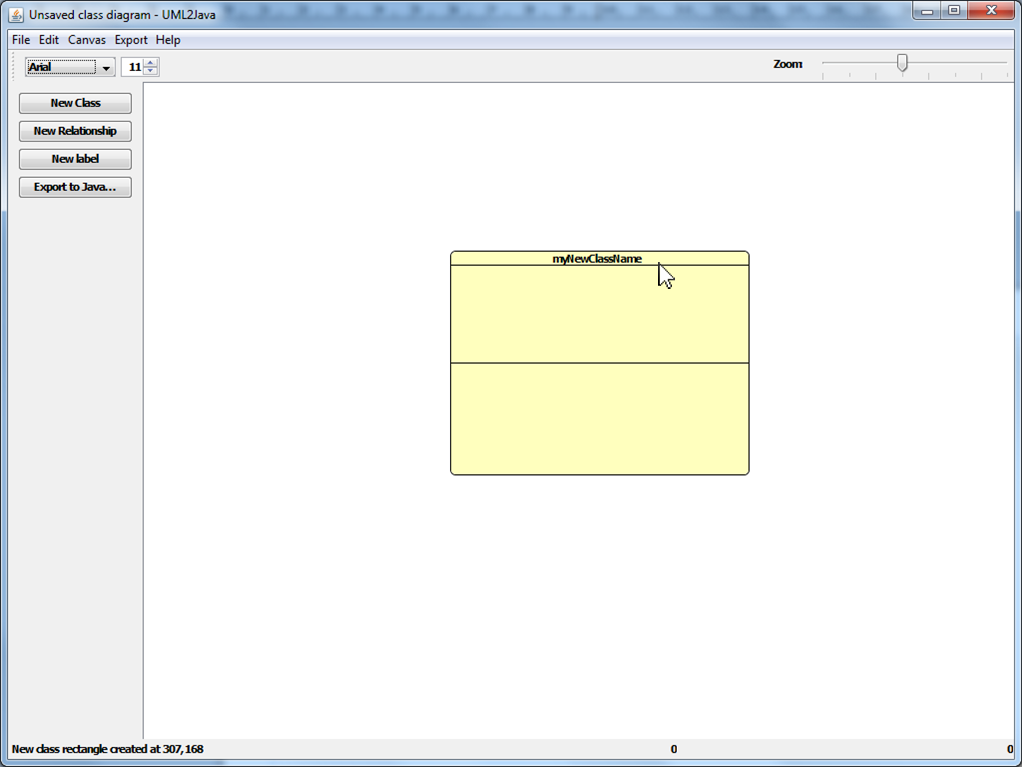
\includegraphics[trim = 135pt 90pt 65pt 70pt, clip, scale=1]{./images/editClassName2.png}}}
\caption{Editing the class name of a Class}
\end{center}
\end{figure}

\subsection{Moving a Class}\index{Editing!Moving the Classes}
To move the classes simply click and hold onto a class and move it to the desired new location on the screen
\begin{figure}[H]
\begin{center}
\subfloat[Click and Hold a class] {\label{fig:editMoveClass1}\fbox{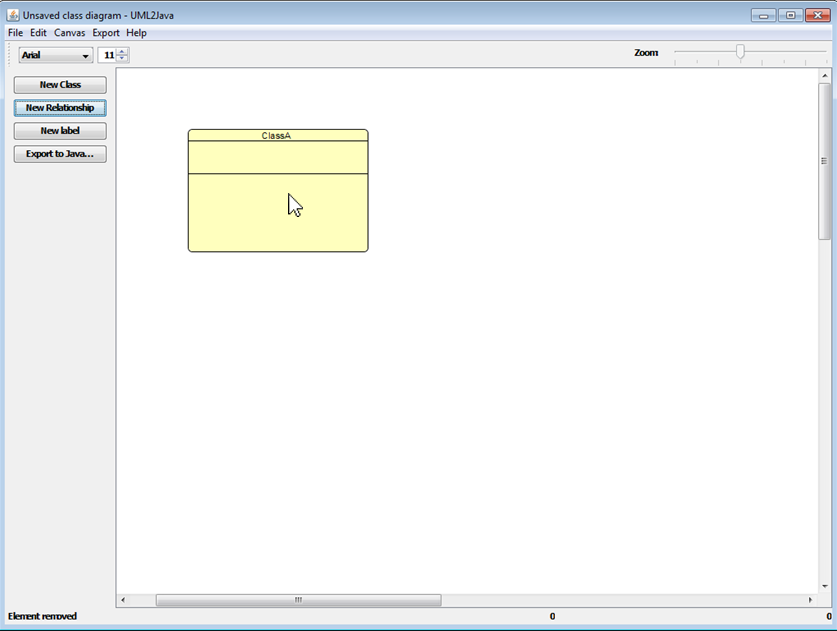
\includegraphics[trim = 0pt 0pt 0pt 0pt, clip, scale=0.6]{./images/edit-moveClass1.png}}} \imagespace
\subfloat[Release at desired location] {\label{fig:editMoveClass2}\fbox{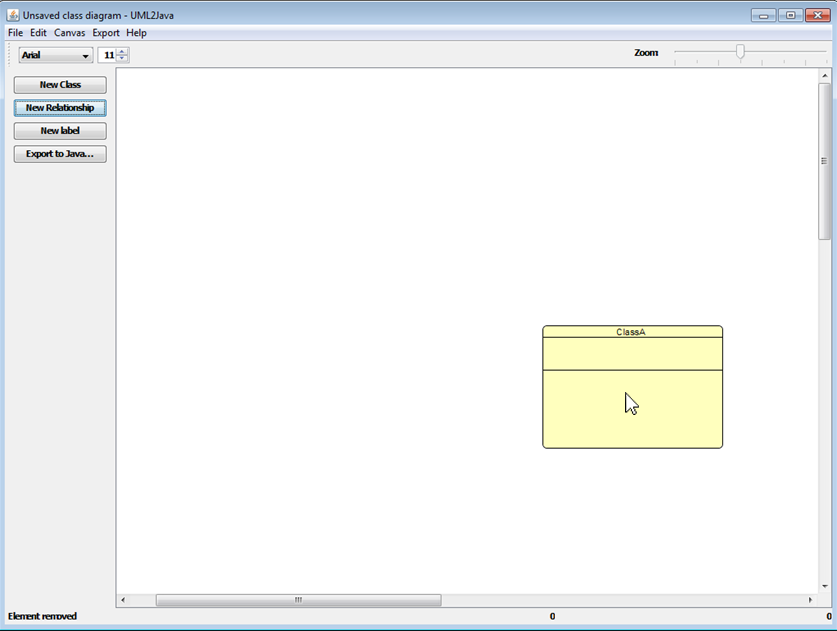
\includegraphics[trim = 0pt 0pt 0pt 0pt, clip, scale=0.6]{./images/edit-moveClass2.png}}}
\caption{Editing a data field in a class}
\end{center}
\end{figure}
\newpage

\subsection{Editing a Data Field}\index{Editing!Data Fields/Variables}
To change a data field in a class added to the diagram \emph{(see Adding new Class \& Adding data fields)} Double-Click the data field you wish to change, the text should highlight and you can then edit the data field, your edit
\textbf{MUST} be in the format\\*
\tab \tab \textbf{(+,-,\#) dataFieldName : DataType}\\*
or if initialised\\* 
\tab \tab \textbf{(+,-,\#) dataFieldName : DataType = initialisation}\\*
Press Return $\hookleftarrow$ to confirm your new Class Name
\begin{figure}[H]
\begin{center}
\subfloat[Double-Click the Class Name] {\label{fig:editDataField}\fbox{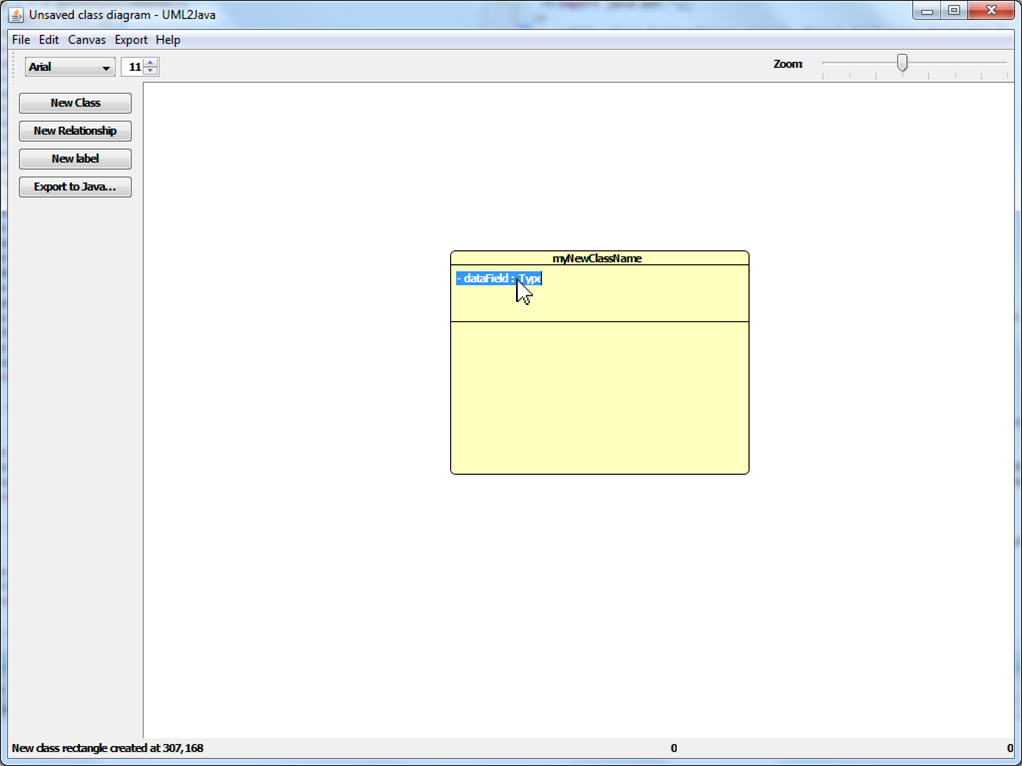
\includegraphics[trim = 135pt 90pt 65pt 70pt, clip, scale=1]{./images/editDataField1.png}}} \imagespace
\subfloat[Changed Name] {\label{fig:editedDataField}\fbox{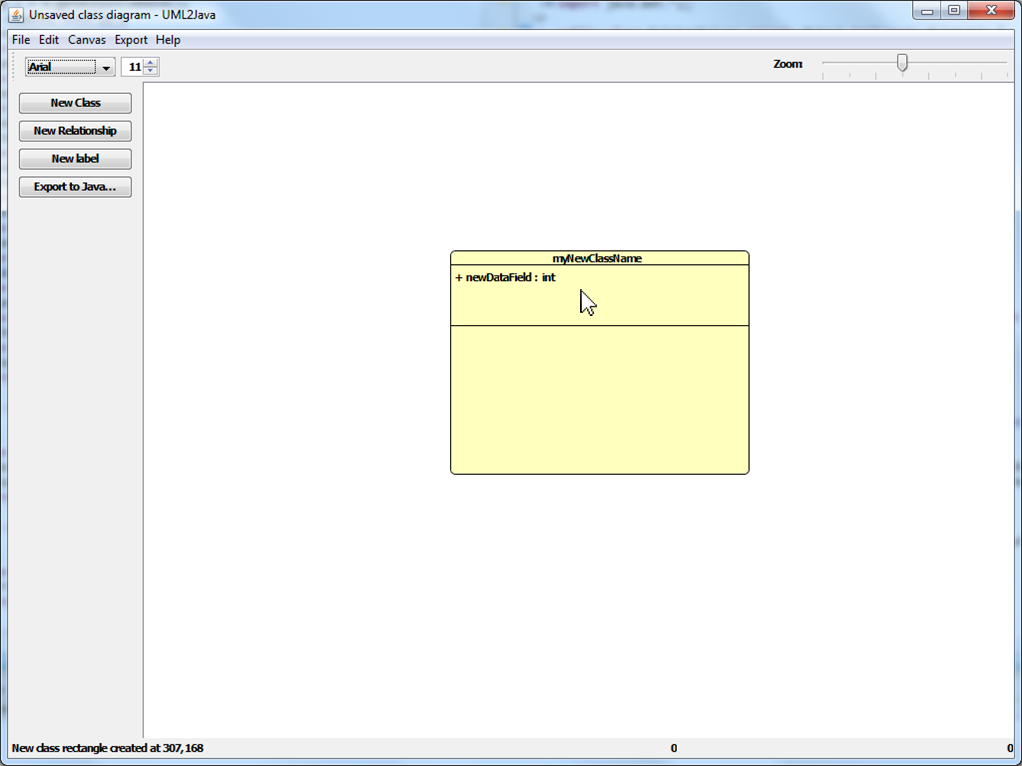
\includegraphics[trim = 135pt 90pt 65pt 70pt, clip, scale=1]{./images/editDataField2.png}}}
\caption{Editing a data field in a class}
\end{center}
\end{figure}

\subsection{Editing a Method in a Class}\index{Editing!Methods}
To change a method in a class added to the diagram \emph{(see Adding new Class \& Adding Methods)} Double-Click the method you wish to change, the text should highlight and you can then edit the method definition, you edit \emph{MUST} be in
the format \\*
\tab \tab \textbf{(+,-,\#) methodName() : Return Type}\\* 
or if arguments are to be passed into the method\\* 
\tab \tab \textbf{(+,-,\#) methodName(arg1 : Arg1Type, arg2 : Arg2Type...) : ReturnType}\\*
Press Return $\hookleftarrow$ to confirm your new Class Name

\begin{figure}[H]
\begin{center}
\subfloat[Double-Click the Class Name] {\label{fig:editMethod}\fbox{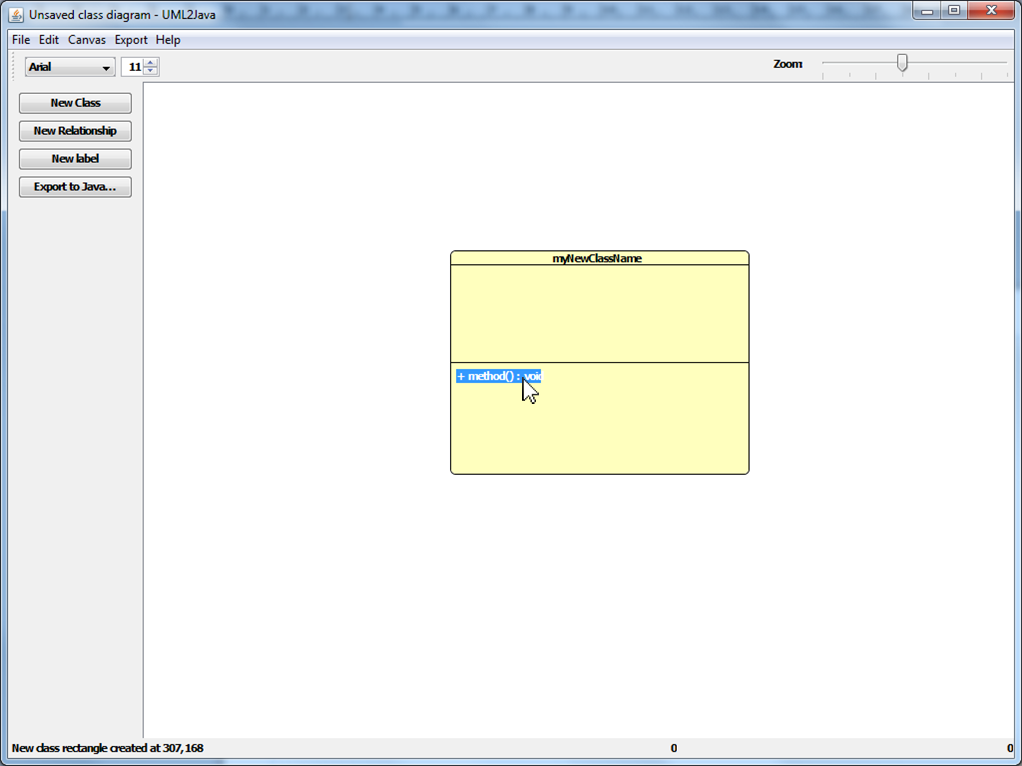
\includegraphics[trim = 135pt 90pt 65pt 70pt, clip, scale=1]{./images/editMethod1.png}}} \imagespace
\subfloat[Changed Name] {\label{fig:editedMethod}\fbox{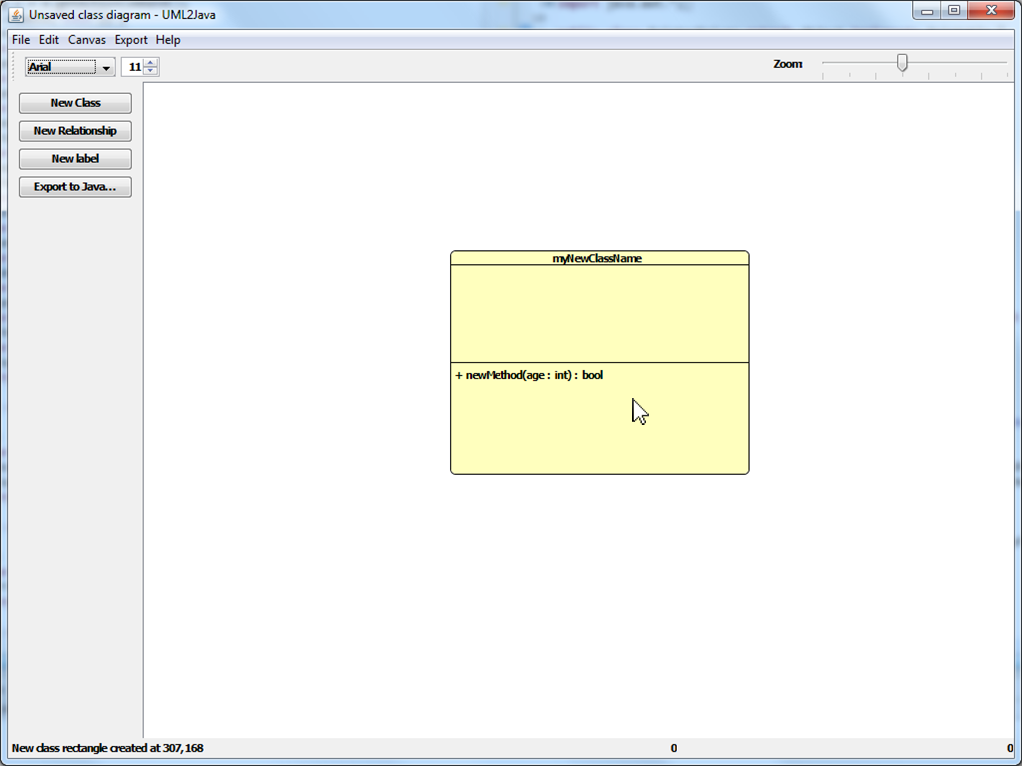
\includegraphics[trim = 135pt 90pt 65pt 70pt, clip, scale=1]{./images/editMethod2.png}}}
\caption{Editing a method in a class}
\end{center}
\end{figure}
\newpage
\subsection{Editing a Relationship}\index{Editing!Relationships}

\subsubsection{Editing the Relationship Type}\index{Editing!Relationships!Relationship Type}
To change the type of relationship between 2 classes, \texttt{Right-Click} on the relationship arrow and hover over \texttt{Change Relationship} and a sub-menu should appear. From this menu you can change the type of relationship, these include: \texttt{Aggregation, Composition, Inheritance, Uses, and Implements}
\vspace{-10pt}
\begin{figure}[H]
\begin{center}
\subfloat[Changing Relationship Type] {\label{fig:changeRelationTyped}\fbox{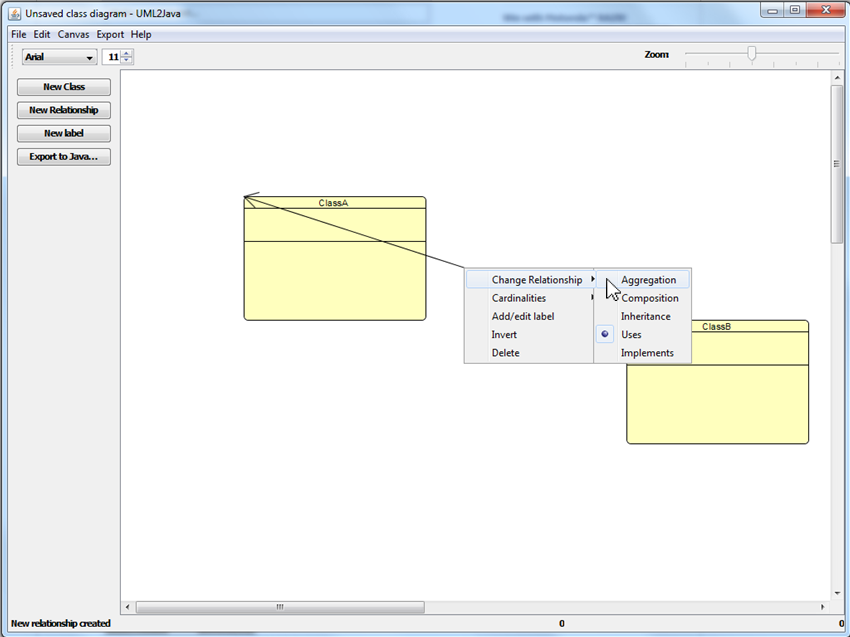
\includegraphics[trim = 200pt 110pt 65pt 110pt, clip, scale=1.3]{./images/edit-relationshiptype1.png}}} \imagespace
\subfloat[Relationship Types] {\label{fig:RelationTypes}\fbox{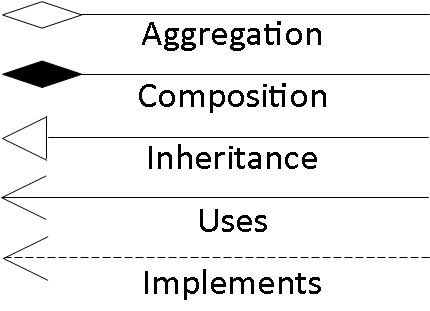
\includegraphics[scale=0.6]{./images/edit-relationshiptype2.png}}}
\caption{Changing Relationship Types}
\end{center}
\end{figure}
\vspace{-20pt}
\subsubsection{Moving Relationship Points}\index{Editing!Relationships!Moving Relationship Points}
You can edit how the relationships look, as by default they snap to the top-left of the class. Simply hover over the end point of a realtionship and green circles will appear over the ends, these will allow you to move the realtionship.
\vspace{-5pt}
\begin{figure}[H]
\begin{center}
\subfloat[Hover over relationship end] {\label{fig:changeRelationTyped}\fbox{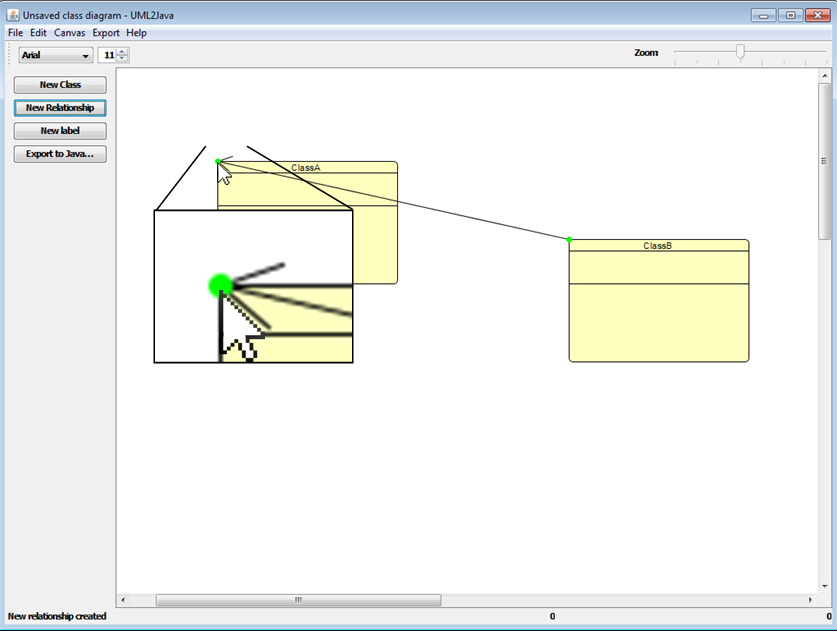
\includegraphics[scale=0.55]{./images/edit-relationshippoint1.png}}} \imagespace
\subfloat[Move to new position] {\label{fig:changeRelationTyped}\fbox{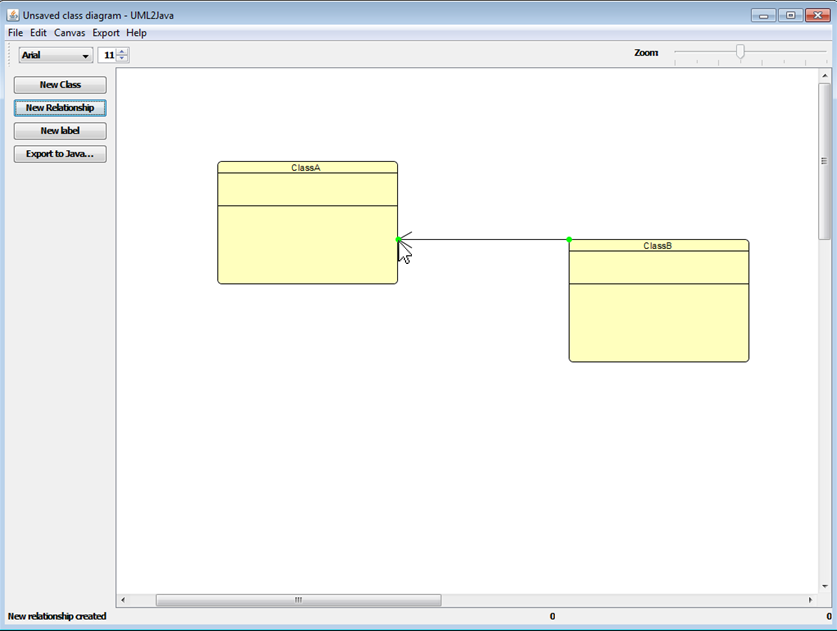
\includegraphics[scale=0.55]{./images/edit-relationshippoint2.png}}}
\end{center}
\vspace{-5pt}
You can also add more points to a relationship, allowing them to change direction to move around other classes where necessary. To do this click and hold at a point on the line and drag to t a new location. This will create a new point that will have a green circle and allow you to move points on the line.
\begin{center}
\subfloat[Creating a new Point] {\label{fig:changeRelationTyped}\fbox{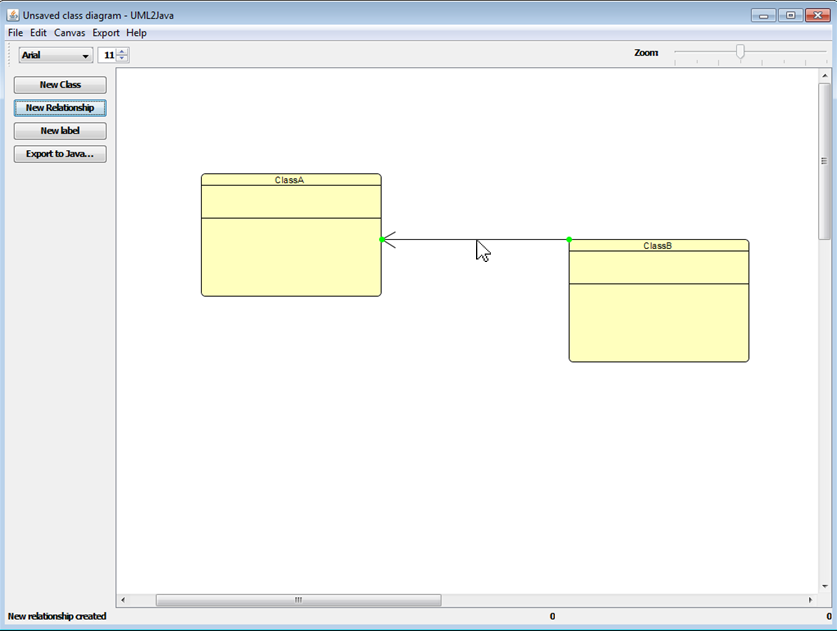
\includegraphics[scale=0.55]{./images/edit-relationshippoint3.png}}} \imagespace
\subfloat[The new line] {\label{fig:changeRelationTyped}\fbox{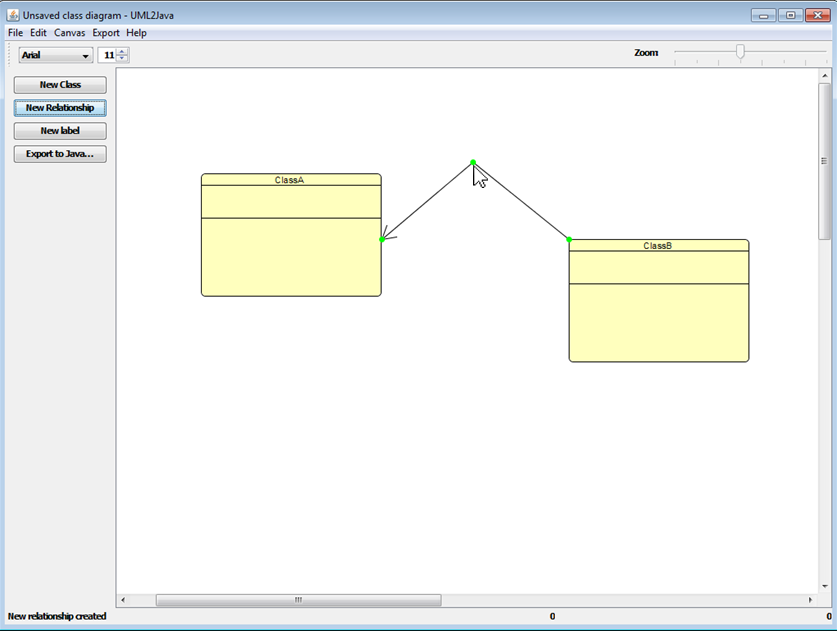
\includegraphics[scale=0.55]{./images/edit-relationshippoint4.png}}}
\vspace{-5pt}
\caption{Moving Relationships and Editing points on the line}
\end{center}
\end{figure}\vspace{-30pt}

\newpage

\subsubsection{Adding a Label to a Relationship}\index{Editing!Relationships!Adding Label}
To add a label to a relationship, \texttt{Right-Click} and select \texttt{Add/Edit Label}. This will allow you to add or edit the current label on the relationship. These are important, as when creating the code files these are used. You can not create labels on Inheritance and Implements relationships \\*
\begin{figure}[H]
\begin{center}
\subfloat[Add/Edit Label] {\label{fig:changeRelationTyped}\fbox{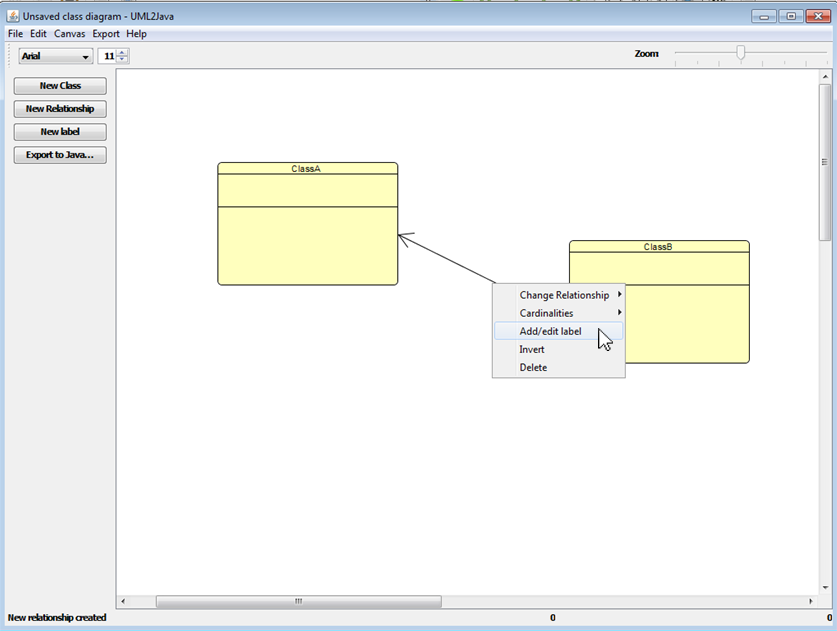
\includegraphics[trim = 200pt 110pt 65pt 110pt, clip, scale=1.3]{./images/edit-relationshiplabeladd.png}}} \imagespace
\subfloat[Editing the Label Name] {\label{fig:changeRelationTyped}\fbox{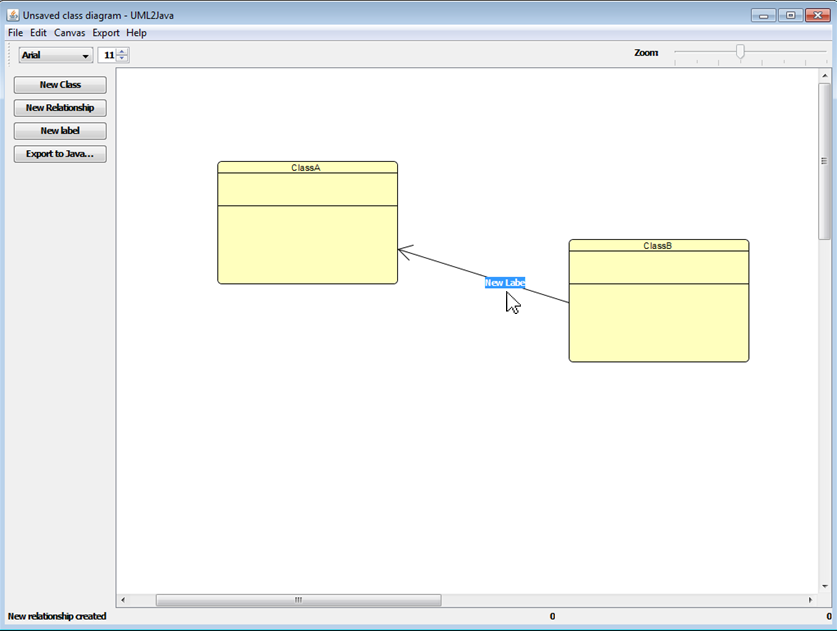
\includegraphics[trim = 200pt 110pt 65pt 110pt, clip, scale=1.3]{./images/edit-relationshiplabeledit.png}}}
\caption{Adding labels to relationships}
\end{center}
\end{figure}

\subsubsection{Adding Cardinalities to the Line}\index{Edit!Adding Cardinalities}
You can add cardinalities to relationships. These include, Zero-to-Many, Many-to-Many and fixed cardinalities. To do this, Right-Click on the relationship and hover over Cardinalities, a sub-menu will appear with 2 options, \texttt{Cardinality From} and \texttt{Cardinality To}. Cardinality From will create the cardinality at the Arrow head side, and Cardinality To will create the open end cardinality. 

\begin{figure}[H]
\begin{center}
\subfloat[Add Cardinalities] {\label{fig:changeRelationTyped}\fbox{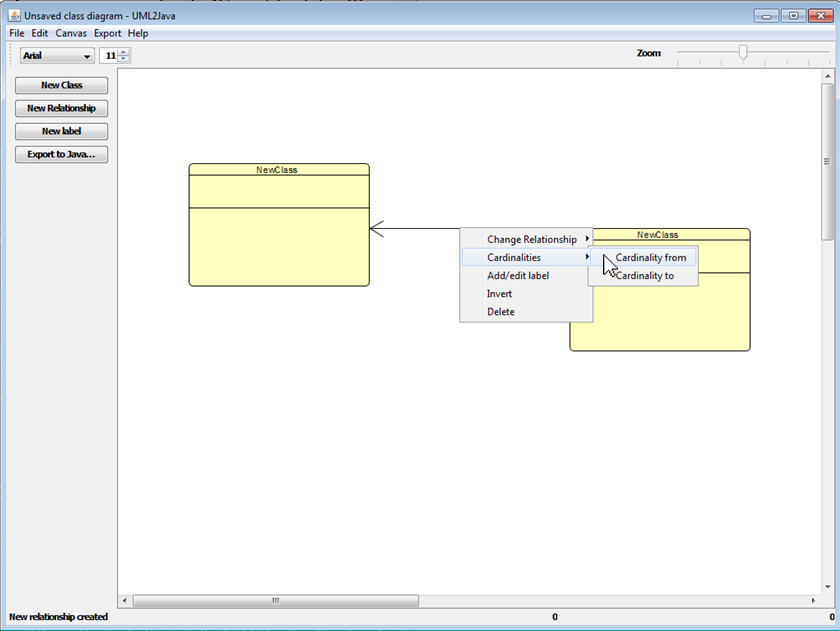
\includegraphics[trim = 200pt 110pt 55pt 90pt, clip, scale=1.3]{./images/edit-addCardinality1.png}}} \imagespace
\subfloat[Created Cardinality] {\label{fig:changeRelationTyped}\fbox{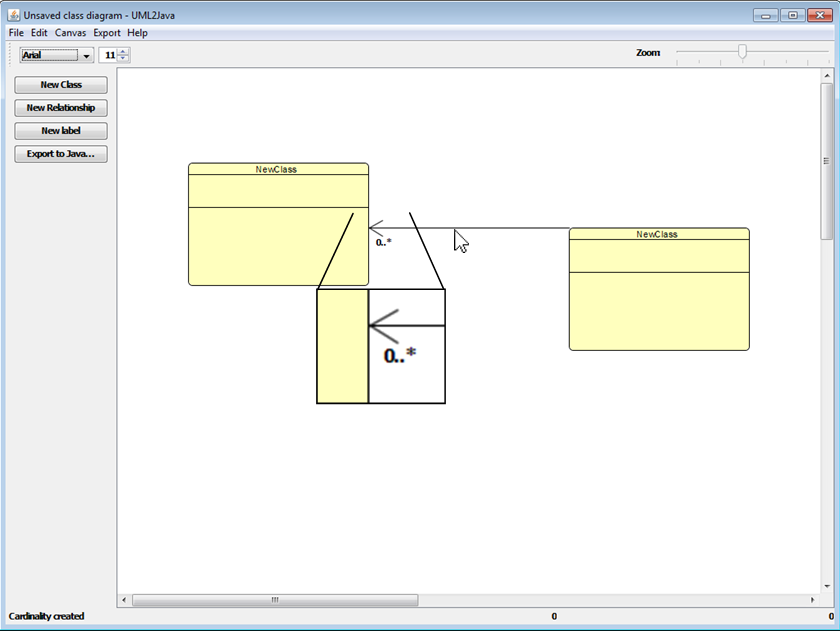
\includegraphics[scale=0.6]{./images/edit-addCardinality2.png}}}
\end{center}
To edit the text, simply double click and this will allow you to edit the text. You will not be able to export the code if cardinalities contain erroneous data, such as words. must either be Whole Numbers or in the form \texttt{\textbf{(\#..\#, or \#..*)}}
\begin{center}
\caption{Adding Cardinalities to relationships}
\end{center}
\end{figure}

\newpage

\listoffigures
\printindex
\end{document}
